\documentclass{report}
\usepackage[utf8]{inputenc}
\usepackage{natbib}
\usepackage{graphicx}
\usepackage{mathtools}
\usepackage{amssymb}
\usepackage{amsfonts}
\usepackage{float}
\usepackage{hyperref}
\usepackage{dsfont}
\newcommand{\N}{\mathbb{N}}
\newcommand{\Pn}{\mathbb{P}}
\newcommand{\indep}{\perp \!\!\! \perp}

\title{Appunti Probabilità e Statistica}
\author{Nicolas Alberti}
\date{Anno Accademico 2020/21}


\begin{document}
\maketitle
\begin{abstract}
    Questi sono appunti redatti seguendo le video-lezioni. \\
    Dovrebbero contenere tutto, quindi dovrebbero essere pronti per lo studio finale.
\end{abstract}
\tableofcontents

\chapter{Lezione 1}

\section{Spazio di Probabilità}

\subsection{Definizione:}

Uno spazio di probabilità è una terna (\(\Omega\), F, P) dove:

\begin{itemize}
    \item \(\Omega\): è un Insieme
    \item F: è una famiglia di sottoinsiemi di \(\Omega\) con una particolare struttura detta \(\sigma\)-algebra
    \item P: da F \(\xrightarrow{}[0, 1]\), è una mappa con misura positiva e normalizzata
\end{itemize}

Descriviamo ora nel particolare il primo simbolo.
\(\Omega\) è lo \textbf{spazio campionario}, ovvero è l'insieme di \textbf{tutti gli esiti} dell'esperimento aleatorio che stiamo considerando.
    \paragraph{Oss.1 :} bisogna scegliere un insieme \(\Omega\) sufficientemente ricco capace di contenere tutti i risultati dell'esperimento considerato. Quindi la scelta dello spazio campionario \textbf{non è} univoca. \\
    \paragraph{Oss.2 :}\begin{itemize}
        \item Se \((\Omega)\) \(\leq\) \(\mathrm{N}\), si dice che lo spazio campionario è \textbf{discreto}.
        \item Se \((\Omega\)) \(\geq\) \(\mathrm{N}\), si dice che lo spazio campionario è \textbf{continuo}.
    \end{itemize}
\subsection{Esempi:}
\begin{enumerate}
    \item Lancio 1 moneta, osservo la faccia uscita: 
    \[\Omega = \{T,C\}\] dove T e C sono Testa e Croce
    \item Lancio 1 moneta per 3 volte, vado a contare il numero di Teste uscite: 
    \[\Omega = \{0, 1, 2, 3\}\]
    \item Lancio 1 moneta per 3 volte, ora osservo la sequenza delle facce ottenute:
    \[\Omega = \{TTT, TTC, TCT, CTT, TCC, CTC, CCT, CCC\}\]
    \item Lancio di 1 moneta fino a che non ottengo Testa e conto il numero di lanci effettuati: 
    \[\Omega = \mathrm{N+} = \{1, 2, 3, ...\}\]
    \item Considero il tempo di vita di un Hard Disk:
    \[\Omega = \mathrm{R+} = [0, +\infty]\]
\end{enumerate}
\subsection{Esiti ed Eventi:}
Esiti ed Eventi sono degli \textbf{elementi speciali} dei sottoinsiemi.
\begin{itemize}
    \item se \(\omega\) \(\in\) \(\Omega\) (ovvero \(\omega\) è \textbf{elemento} di \(\Omega\)), allora è detto \textbf{esito} (o \textit{evento elementare}
    \item se E \(\subseteq\) \(\Omega\) (ovvero E è \textbf{sottoinsieme} di \(\Omega\), allora è detto \textbf{evento} 
\end{itemize}

Se l'esecuzione dell'esperimento dà come risultato \(\omega\) \(\in\) \(\Omega\), diremo che si è verificato \(\omega\). \\

Per ogni E tale che \(\omega\) \(\in\) E, allora diremo che si è verificato E.

\subsection{Esempio:}
Riprendiamo l'esempio 3 descritto prima. Lo spazio campionario che rappresenta i possibili risultati di 3 lanci di una moneta è : \[\Omega = \{TTT, TTC, TCT, CTT, TCC, CTC, CCT, CCC\}\]

Gli eventi possibili saranno quindi:
\begin{itemize}
    \item \(E_k\) = "ottengo K croci (in 3 lanci) ", con K = 0, 1, 2, 3
    Per ogni K devo esaminarne gli eventi \textbf{favorevoli}:
    \begin{enumerate}
        \item \(E_0\) = {TTT}
        \item \(E_1\) = {TCT, CTT, TTC}
        \item \(E_2\) = {TCC, CTC, CCT}
        \item \(E_3\) = {CCC}
    \end{enumerate}
    Supponiamo di avere ottenuto come esito, dopo i 3 lanci, CTC: si verifica quindi \(E_2\) ma non si verificano \(E_0\), \(E_1\) ed \(E_3\).
\end{itemize}

\subsection{Eventi banali ed onnipresenti:}
Sono 2 e sono quelli di seguito:
\begin{itemize}
    \item \(\Omega\): evento \textbf{certo}
    \item \(\emptyset\): evento \textbf{impossibile}
\end{itemize}

\section{Operazioni elementari sugli eventi}

Le operazioni insiemistiche permettono di combinare più spazi campionari, al fine di ottenere eventi più interessanti.

Siano E, F \(\in \Omega\) degli eventi. Abbiamo:
\begin{itemize}
    \item il \textbf{complementare} di E (evento):
    \[E^c = \{(\omega \in \Omega | \omega \ni)E\}\]
    E' l'insieme degli esiti che \textbf{non stanno} in E.
    Probabilisticamente, \(E^c\) si verifica quando non si verifica E.
    \item \textbf{Intersezione} di E con F: \[E \cap F\ =\ \{\omega \in \Omega | \omega \in E\ e\ \omega \in F\}\] Probabilisticamente, \(E \cap F\) si verifica solo se si verificano \textbf{sia E che F}. Se E ed F sono tali che: \[E \cap F\ = \varnothing \] si dice che E ed F sono \textbf{incompatibili} o \textbf{disgiunti}, cioè E ed F non si possono verificare allo stesso momento.
    \item \textbf{Unione} di E con F: \[E \cup F\ =\ \{\omega \in \Omega | \omega\in E\ o\ \omega \in F\}\] Probabilisticamente, \(E \cup F\) si verifica se \textbf{almeno uno} tra E ed F si verifica. L'unione corrisponde ad una \textbf{"o" inclusiva}.
    \item \textbf{Differenza} tra insiemi. Ne esistono di 2 tipi:
    \begin{itemize}
        \item \(E\backslash F\) \textit{(si legge E meno F)} \textbf{non simmetrica}: significa che (\(F\backslash E \neq E\backslash F\)). \[E\backslash F\ = \{\omega \in \Omega\ |\ \omega \in E\ e\ \omega \not\in F\}\]
        Probabilisticamente, si dice che \(E\backslash F\) si verifica quando si verifica E \textbf{ma non si verifica} F.
        \item \(E \triangle F\): è la differenza \textbf{simmetrica}: \[E \triangle F\ =\ \{\omega \in \Omega\ |\ \omega \in (E\backslash F)\ o\ \omega \in (F \backslash E)\}\] Probabilisticamente, si dice che \(E \triangle F \) si verifica se \textbf{esattamente uno} tra E ed F si verifica. Corrisponde ad una \textbf{"o" esclusiva}.
    \end{itemize}
\end{itemize}
\paragraph{Esempio} 
Vediamo l'esempio dei 3 lanci della moneta visto in precedenza. Abbiamo definito: \(E_K\ =\ "Ottengo\ K\ croci",\ K\ =\ 0,1,2,3. \). Abbiamo un evento \[E\ =\ "esce\ almeno\ una\ testa"\ =\ E{^C_3}\] il quale è il \textbf{complementare} di \[F\ =\ "escono\ almeno\ 2\ croci"\ =\ E_2 \cup E_3\] Abbiamo anche l'evento \[G\ =\ "escono\ almeno\ due\ teste"\ =\ (E_2 \cup E_3)^C\]
\section{Proprietà fondamentali di unione ed intersezione}
Esistono varie leggi
\begin{itemize}
    \item Leggi \textbf{commutative} \[E \cup F\ =\ F \cup E\] ed anche \[E \cap F\ =\ F \cap E\]
    \item Leggi \textbf{associative} \[(E \cup F) \cup G\ =\ E \cup (F \cup G)\] ed anche \[(E \cap F)\cap G\ =\ E \cap (F \cap G)\]
    \item Leggi \textbf{distributive} \[E \cup (F \cap G)\ =\ (E \cup F)\cap (E \cup G)\] ed anche \[E \cap (F \cup G)\ =\ (E \cap F)\cup (E \cap G)\]
    \item Leggi di \textbf{De Morgan} \[(E \cup F)^C\ =\ E^C \cap F^C\] ed anche \[(E \cap F)^C\ = E^C \cup F^C\ \]
\end{itemize}

\section{Decomposizioni in unioni disgiunte}
E' un metodo conveniente quando si tratteranno le probabilità. Dobbiamo innanzitutto \textbf{ripartire lo spazio campionario}.
\begin{itemize}
    \item \textbf{Partizione di \(\Omega\)}: E' una famiglia di eventi \(\{E_N\}_{N\geq1}\). Gli eventi sono \textbf{a 2 a 2 disgiunti} e la proprietà è anche detta \textit{mutua disgiunzione} o \textit{mutua incompatibilità} e la loro unione porta ad ottenere lo spazio campionario \(\Omega\) di partenza. Simbolicamente diciamo:
    \begin{itemize}
        \item \(E_i \cap E_j = \varnothing\) per \(i \neq j\)
        \item \(\bigcup_{N\geq 1} E_N = \Omega\)
    \end{itemize}
    Significa che fra gli eventi \textbf{non deve esserci intersezione} e quando verranno riuniti essi copriranno \textbf{tutto lo spazio campionario}.

\paragraph{Esempi} \begin{enumerate}
    \item Se \(E \subseteq \Omega\) è un evento, allora la famiglia \(\{E, E^C\}\) è una partizione di \(\Omega\).
    \item Prendiamo di nuovo l'esempio dei 3 lanci di una moneta. La famiglia che costruiamo con gli eventi \(E_K = \{E_0,E_1,E_2,E_3\}\) (che, ricordiamo, sono l'ottenimento di K croci), questa famiglia \textbf{è una partizione di} \(\Omega\).
\end{enumerate}
\item \textbf{Decomposizione di un evento rispetto ad una partizione}: Siano F evento e \(\{E, E^C\}\) una partizione di \(\Omega\). Allora \[F = (F \cap E) \cup (F\cap E^C)\] Possiamo dire che \((F \cap E)\ e\ (F\cap E^C)\) sono eventi \textbf{disgiunti}.
\clearpage
\begin{figure}[hb]
    \centering
    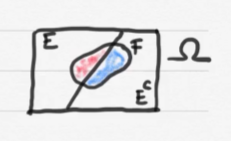
\includegraphics[width = 6cm]{EventiDisgiuntiinOmega.png}
    \caption{Questa è la rappresentazione grafica di ciò che abbiamo appena descritto}
    \label{fig:EventiDisgiunti}
\end{figure}
In generale, se \(\{E_n\}_{n\geq 1}\) è una partizione di \(\Omega\), abbiamo \[F = \bigcup_{n\geq 1} (F \cap E_n)\]

\item \textbf{Decomposizione dell'unione di due eventi}: serve a riscrivere un unione in modo che gli eventi che vado ad unire per rappresentarla siano \textbf{a due a due disgiunti}. Non esiste una regola ed esistono varie decomposizioni. Siano \[E,F \subseteq \Omega\ eventi\] si può avere il primo caso (\ref{fig:DecomposizioneC1})\[E \cup F = (E \backslash F)\cup (E \cap F)\cup (F\backslash E)\]
Altrimenti possiamo avere anche il secondo caso (\ref{fig:DecomposizioneC2}): \[E \cup F = E \cup (F \backslash E)\]
\begin{figure}
    \centering
    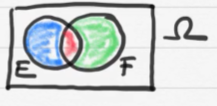
\includegraphics[width = 6cm]{DecomposizioneC.png}
    \caption{Ecco la raffigurazione del primo esempio di decomposizione: la parte blu indica \((E\backslash F)\), la parte rossa indica \((E \cap F)\) mentre la parte verde indica \((F\backslash E)\). Interessante notare come questi tre eventi siano anche \textbf{disgiunti} tra loro.}
    \label{fig:DecomposizioneC1}
\end{figure}
\begin{figure}
    \centering
    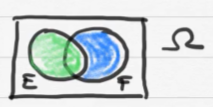
\includegraphics[width = 6cm]{DecomposizioneC2.png}
    \caption{Ecco la raffigurazione del secondo esempio. In verde abbiamo E, mentre in blu abbiamo \((F \backslash E)\). Questi due eventi restano \textbf{disgiunti}.}
    \label{fig:DecomposizioneC2}
\end{figure}
\end{itemize}

\chapter{Lezione 2}
\section{La sigma-algebra degli Eventi}
Una famiglia \textit{F} (ricorda F corsivo) di sottoinsiemi di \(\Omega\) si chiama \(\sigma-algebra\) se: \begin{enumerate}
    \item \textit{F} \textbf{è non vuota}
    \item se \(E \in \textit{F}\), allora \(E^C \in F\)
    \item se \(E_n \in \textit{F}\) per \(n \geq 1\), allora \(\bigcup_{n \geq 1} E_n \in F\); identifica la chiusura per unione numerabile.
\end{enumerate}
\subsection{Esempi}
Vediamo alcuni esempi: \begin{enumerate}
    \item \(\sigma-algebra\) \textbf{banale}: qualunque sia \(\Omega\), la famiglia \(\{\Omega, \varnothing\}\) è una \(\sigma-algebra\). E' quindi \(\sigma-algebra\) lo spazio campionario \(\Omega\) e lo spazio vuoto \(\varnothing\).
    \item \(\sigma-algebra\) \textbf{generata da un evento}: dato \(\Omega\) e un evento \(E \subseteq \Omega\), la famiglia \(\{\varnothing, E, E^C, \Omega\}\) è una \(\sigma-algebra\).
    \item \(\sigma-algebra\) \textbf{massima}: qualunque sia \(\Omega\), la famiglia di tutti i suoi sottoinsiemi (detta \textbf{insieme delle parti}) \[\textit{F} = \Pn(\Omega)\] è una \(\sigma-algebra\). E' la più grande \(\sigma-algebra\) costruibile. \paragraph{Nota:} se \(\Omega\) è discreto, prenderemo sempre \(\textit{F} = \Pn(\Omega)\) 
\end{enumerate}
\subsection{Conseguenze elementari degli assiomi}
Vediamo alcune conseguenze degli assiomi appena descritti: \begin{enumerate}
    \item \(\Omega \in \textit{F}\ e\ \varnothing \in \textit{F}\)\\ Come lo vediamo? Esiste un \(E \in \textit{F}\) per la condizione 1. vista prima, ciò implica \(\longrightarrow E^C \in \textit{F}\) per la condizione 2. di prima.\\ 
    Ora vediamo \(\Omega = \{E \cup E^C\} \in \textit{F}\), poichè la loro unione determina un numero \textbf{finito} di elementi, dato dalla condizione 3. vista prima. In conclusione diciamo anche che \(\Omega \in \textit{F}\) e anche che \(\varnothing = \Omega^C \in \textit{F}\) per la condizione 2.
    \item Chiusura per \textbf{intersezione numerabile}: dice che se ho \(E_n \in \textit{F}\) per ogni \(n \geq 1\), allora anche \(\bigcap_{n \geq 1}E_n \in \textit{F}\) sarà nella \(\sigma-algebra\).\\
    Come la vediamo? Devo riscrivere questa intersezione in un modo che mi permetta di utilizzare tutte le informazioni che ho, che sono solo su \textbf{unione e complementazione} di eventi sulla \(\sigma-algebra\). Sfrutto le \textbf{Leggi di De Morgan}: \begin{itemize}
        \item \((\bigcap_{n \geq 1}E_n)^C\ = \bigcup_{n \geq 1}E_n^C\ \in \textit{F}\).\\ Gli \(E_n^C \in \textit{F}\) per la \textbf{condizione 2.}. La loro \textbf{unione numerabile} \(\in \textit{F}\) per la \textbf{condizione 3.}
        \item Chiudiamo dicendo: \(\bigcap_{n \geq 1}E_n = ((\bigcap_{n \geq 1}E_n)^C)^C\) dove la \textbf{prima intersezione} complementare \(\in \textit{F}\)per il primo punto di questo elenco, ed il \textbf{suo complementare} \(\in \textit{F}\) per la \textbf{condzione 2.} della definizione precedente. Quindi l'oggetto è un elemento della \(\sigma-algebra\).
    \end{itemize}
\end{enumerate}
\section{Misura di Probabilità P}
\paragraph{Definizione} Una misura di probabilità è una \textbf{mappa} \[P: \textit{F} \longrightarrow [01]\] in cui \[E \longmapsto P(E)\] dove \(P(E)\) è la probabilità dell'evento E, tale che soddisfi 2 proprietà: \begin{enumerate}
    \item \(P(\Omega) = 1\), è la \textbf{normalizzazione}
    \item se \(\{E_n\}_{n \geq 1}\) famiglia di eventi \textbf{mutualmente incompatibili} (ovvero\\ quando l'intersezione fra i,j di una famiglia è vuota quando \(i \neq j\)), allora \[P(\bigcup_{n \geq 1}E_n) = \sum_{n \geq 1} P(E_n)\]
\end{enumerate}
La misura, come detto nella prima lezione, deve essere \textbf{positiva e normalizzata}. \begin{itemize}
    \item La \textbf{positività} è implicita nel fatto che la probabilità prende \textbf{valori nell'intervallo [0,1]}, quindi certamente positivi
    \item La condizione di \textbf{normalizzazione} invece è la condizione sulla probabilità dell'\textbf{intero spazio campionario}, come indicato prima.
\end{itemize}
\subsection{Conseguenze elementari degli assiomi}
\begin{enumerate}
    \item \(P(E^C) = 1-P(E)\): come lo vediamo?\\
    Si ha che \(1 = P(\Omega) = P(E \cup E^C) =^{per\ condizione\ 2\ definizione} P(E) + P(E^c)\), dove \(E\ ed\ E^c\) sono \textbf{disgiunti}.\\
    Da cui quindi otteniamo \[P(E^c) = 1 - P(E)\]
    \item \(P(\varnothing) = 0\): come lo vediamo?\\
    Si ha \(\varnothing = \Omega^c\), quindi posso usare la prima proprietà appena definita per dire: \[P(\varnothing) = P(\Omega^c) =^{(per\ proprieta'\ 1)} 1 - P(\Omega)_{(= 1\ per\ condizione\ 1)} = 0\]
    \item Se \(E \subset F\), allora \(P(E) < P(F)\): come lo vediamo?\\
    Se \(E \subset F\), allora \(F = E \cup (F\backslash E)\), dove i due eventi che sto unendo sono \textbf{disgiunti}. Quindi \[P(F) =^{(per\ proprieta'\ 2\ Misura\ delle\ Probabilita')} P(E) + P(F\backslash E)\] %disegno
    \(P(F\backslash E) \in [0,1]\), che è \textbf{positivo}, da cui segue \[P(F) > P(E)\] 
    \item Formula di \textbf{inclusione/esclusione}: ci dà modo di calcolare la probabilità di una \textbf{unione di eventi}.
    \[P(E \cup F) = P(E) + P(F) - P(E \cap F)\] Come la vedo?\\
    Si ha \(E \cup F = E \cup (F\backslash E)\) (unione disgiunta) e quindi \(P(E \cup F) = P(E) + P(F\backslash E)\).\\
    Inoltre \(F = (F\backslash E) \cup (F \cap E)\) (unione disgiunta) e quindi \(P( F) = P(F\backslash E) + P(F \cap E)\).\\
    Ricavo che: \(P(F\backslash E) = P(F) - P(F \cap E)\). Lo sostituisco nella probabilità dell'unione scritta inizialmente ed ottengo: \[P(E \cup F) = P(E) + P(F) - P(F \cap E) \]
\end{enumerate}
\subsection{Osservazione:} Dato (\(\Omega, \textit{F}\)) per completare la terna, la scelta della misura di probabilità P \textbf{non è univocamente determinata}, poichè gli assiomi \textbf{non determinano} un' unica misura di probabilità.
\paragraph{Esempio:} Consideriamo il lancio di una moneta: \[\Omega = \{T,C\}\ e\ \textit{F} = \Pn(\Omega)\]
Abbiamo \textbf{infinite} misure di probabilità compatibili con gli assiomi: \[(T) = p \in [0,1]\ ,\ P(C) = 1 - p\]
\chapter{Lezione 3}
\section{Scelta della Misura di Probabilità P}
\subsection{Scelta di P nel caso di Omega Discreto}
Consideriamo \((\Omega, \textit{F}, P)\), con \(\Omega\) discreto e \(\textit{F} = \Pn(\Omega)\). Come si assegna P su \textit{F}?\\
Se \(\Omega = \{\omega_1, \omega_2, ... \}\) è discreta, allora ogni evento \(E \subseteq \Omega\) (o, equivalentemente \(E \in \textit{F}\)) può essere scritto come \textbf{unione numerabile (o finita)} di elementi di \(\Omega\), cioè significa che: \[E = \{\omega_{i1}, \omega_{i2}, \omega_{i3}, ...\} = \{\omega_{i1}\} \cup \{\omega_{i2}\} \cup \{\omega_{i3}\} \cup ...\] (dove gli indici \textit{i} sono scelti precisamente) è una \textbf{unione disgiunta di singoletti}.\\
Se P fosse la probabilità a cui siamo interessati, allora avremmo che \[P(E) = P(\{\omega_{i1}) + P(\{\omega_{i2}) + P(\{\omega_{i3}) + ...\}\]
Se leggiamo dal \textbf{punto di vista opposto}: è sufficiente assegnare \[P(\{\omega_{i}\}) = p_i\] con i = 1, 2, 3, ... tali che: \begin{itemize}
    \item \(p_i \in [0, 1]\), quindi la \textbf{positività}
    \item \(\sum_{i \geq 1} p_i = 1\), quindi la \textbf{normalizzazione}
\end{itemize}
Quindi se \(\Omega\) è discreto, assegno le \textbf{proprietà ai singoletti} che poi andrò ad \textbf{unire} per ottenere la probabilità dell'evento P.
\subsubsection{Esempio}
Consideriamo \(\Omega = \N\) e definiamo \(P(\{i\}) = \frac{1}{2^i} \) per ogni \(i \in \N\). Questa è \textbf{una misura di probabilità}. Infatti verifico: \begin{itemize}
    \item \(0 < \frac{1}{2^i} \leq 1\)
    \item \(\sum_{\frac{1}{2^i}} = -1 + \sum_{i \geq 0}\frac{1}{2^i} = -1 + \frac{1}{1 - \frac{1}{2}} = 1 \)\\ 
    (Piccolo ripasso \textbf{serie geometrica}: \(\sum_{K \geq 0}x^K\), dove x è detta \textbf{ragione}, abbiamo che: \begin{itemize}
        \item \textbf{converge} se \(0 < x < 1\)
        \item \textbf{diverge} altrimenti
    \end{itemize}
    Se converge \(\sum_{K \geq 0}x^K = \frac{1}{1-x}\))
\end{itemize}
Possiamo utilizzare questa misura di probabilità per calcolare la probabilità dell'insieme dei multipli di 3 . Si ha infatti: \[P(\{3, 6, 9, 12, ...\}) = P(\{3*i\ con\ i \in \N\}) = \] \[= \sum_{i \geq 1} \frac{1}{2^{3i}} = \sum_{i \geq 1} \frac{1}{8^i} = -1 + \sum_{i \geq 0} \frac{1}{8^i} = -1 + \frac{1}{1 - \frac{1}{8}} = \frac{1}{7}\]
\subsection{Scelta di P nel caso di Omega Finito}
Se \(\Omega = \{\omega_1, \omega_2, ..., \omega_N\}\) ha \textbf{cardinalità finita} \(\N\), possiamo scegliere la \textbf{misura di probabilità uniforme}, detta uniforme poichè assegna a \textbf{tutti gli esiti la stessa probabilità}, ovvero: \[P(\{\omega_1\}) = P(\{\omega_2\}) = ... = P(\{\omega_N\}) = \frac{1}{N}\] Questo mi dice che \textbf{tutti} gli esiti sono \textbf{equiprobabili}.\\
Lo spazio di probabilità che ottengo scegliendo \(\Omega finito, \sigma-algebra\ delle\ parti\) e spazio di probabilità uniforme è detto \textbf{spazio di probabilità uniforme}. Come faccio a calcolare la probabilità di un evento E?\\
Per ogni evento \(E \in \textit{F}\), si ha \[P(E) = \sum_{\omega_i \in E} P(\{\omega_i\}) = |E| * \frac{1}{N} = \frac{|E|}{|\Omega|}\] (ovvero cardinalità di E fratto cardinalità di Omega). Questa ultima dicitura indica la famosa descrizione: \[\frac{Casi\ Favorevoli}{Casi\ Possibili}\]
\subsubsection{Esempio}
Consideriamo un mazzo di carte da poker (52 carte) e peschiamo una carta. \begin{itemize}
    \item La probabilità di estrarre una regina è \(\frac{4}{52}\)
    \item La probabilità di estrarre una carta di cuori è \(\frac{13}{52}\)
    \item La probabilità di estrarre la regina di cuori è \(\frac{1}{52}\) 
\end{itemize}
\subsubsection{Esercizio}
Lanciamo due dadi equilibrati. \begin{enumerate}
    \item \(E_1 =\) "Qual è la probabilità che la somma dei punteggi sia 8?" 
    \item \(E_2 =\) "Qual è la probabilità che escano due punteggi uguali?"
    \item \(E_3 =\) "Qual è la probabilità di ottenere 8 con due dadi con lo stesso punteggio?"
\end{enumerate} 
\paragraph{Soluzione} Lo spazio campionario è \[\Omega = \{(i, j):\ i,j \in \{1, 2, ..., 6\}\}\] cioè l'insieme delle coppie dei punteggi ottenuti sui due dadi.
Si ha \(|\Omega| = 6*6 = 36\)
\begin{enumerate}
    \item Consideriamo l' evento \[E_1 = \{(2,6), (3,5), (4,4), (5,3), (6,2)\}\] si ha \[P(E) = \frac{|E|}{|\Omega|} = \frac{5}{36}\]
    \item Consideriamo l'evento \[E_2 = \{(1,1), (2,2), (3,3), (4,4), (5,5), (6,6)\}\] si ha \[P(E) = \frac{|E|}{|\Omega|} = \frac{6}{36}\]
    \item Consideriamo l'evento \[E_3 = E_1 \cap E_2 = \{(4,4)\}\] si ha \[P(E) = \frac{|E|}{|\Omega|} = \frac{1}{36}\]
\end{enumerate}
\paragraph{Punto chiave:} Il punto chiave è il \textbf{contare gli elementi di un insieme}.
\section{Combinatoria Elementare}
\subsection{Principio Fondamentale del Conteggio (P.F.C)}
Sia E un insieme. Supponiamo che ogni elemento di E \textbf{si possa determinare univocamente mediante K scelte }successive, tali che: \begin{itemize}
    \item La prima scelta ha \(n_1\) esiti possibili
    \item La seconda scelta ha \(n_2\) esiti possibili
    \item La \textbf{K-esima} scelta ha \(n_k\) esiti possibili
\end{itemize}
allora la cardinalità di E sarà: \[|E| = n_1*n_2*...*n_k\]
\subsubsection{Esempio}
Contiamo le carte in un mazzo da poker, usando il P.F.C. Ogni carta del mazzo è individuata da un seme (C, Q, F, P) e da un valore (A, 2, 3, ..., J, Q, K). Per individuare una carta, cosa faccio? \begin{enumerate}
    \item Scelgo il \textbf{seme}: \textbf{4 esiti possibili}
    \item Scelgo il \textbf{valore}: \textbf{13 esiti possibili}
\end{enumerate}
Quindi otteniamo che il numero di carte nel mazzo è: \[4*13 = 52\]
\paragraph{Osservazione} Cosa vuol dire "determinare univocamente"? Vuol dire che \textbf{sequenze distinte di scelte individuano elementi diversi di E}.\\ 
E' importante, perchè \textbf{se non è soddisfatta} la cardinalità risulterà \textbf{errata!} e il P.F.C non varrà.
\subsubsection{Esempio 2}
Si deve formare un comitato di 2 persone da scegliersi dal gruppo \(\{U, D_1, D_2\}\) (dove U = Uomo e D = Donna). I possibili comitati sono 3: \begin{enumerate}
    \item \(\{U, D_1\}\)
    \item \(\{U, D_2\}\)
    \item \(\{D_1, D_2\}\)
\end{enumerate}
Ora ragioniamo come segue. Scegliere un comitato equivale a fare le seguenti scelte: \begin{enumerate}
    \item Scelgo una delle due donne: ho 2 esiti possibili
    \item Scelgo la persona che manca tra i rimanenti: ho 2 esiti possibili.
\end{enumerate}
Applico il P.F.C ed ottengo che il numero dei comitati è \(2*2 = 4\), ma \textbf{in realtà} i comitati \textbf{sono solo 3}. Dove sta l'errore?\\
Sta nel fatto che ci sono \textbf{2 distinte sequenze di scelte} che mi danno come risultato il comitato \(\{D_1, D_2\}\) e sono: \begin{itemize}
    \item \(\{D_1, D_2\}\)
    \item \(\{D_2, D_1\}\)
\end{itemize}
\chapter{Lezione 4}
\section{Disposizioni con Ripetizione}
\paragraph{Scopo:} Contare le K-uple \textbf{ordinate} che posso creare scegliendo ogni entrata da n oggetti con la possibilità di ripetizione.\\
Ogni entrata può essere scelta tra \textbf{n alternative} (ci può essere \textbf{ripetizione}) e faccio \textbf{K scelte} totali, una per ogni entrata del vettore che voglio costruire. Quindi, per sapere il numero totale di disposizioni con ripetizione è \[n^K\]
\subsubsection{Esempi}
\begin{enumerate}
    \item Una cassaforte con codice a 7 cifre ha \(10^7\) codici possibili.
    \item Metodo per generare sottoinsiemi di un dato insieme: se E è un insieme \textbf{finito}, con cardinalità \textbf{K}, allora i possibili sottoinsiemi di E sono \[2^K\]
    Infatti, possiamo specificare un sottoinsieme F di E nel seguente modo: ad ogni elemento di F possiamo assegnare:\begin{itemize}
        \item Il valore \textbf{1} se \textbf{sta in F}
        \item Il valore \textbf{0} se \textbf{non sta in F}
    \end{itemize}
    Ogni stringa di bit \(\{0, 1\}\) di lunghezza K \textbf{codifica un sottoinsieme di E}.\\
    \paragraph{Esempio:} E = \(\{+, -, *, :\}\), \(|E| = 4\) con stringa di bit: 0101 che genera il sottoinsieme: \[\{-, :\}\] poichè i valori corrispondono esattamente agli elementi in E \(("+" = 0\ quindi\ no, "-" = 1\ quindi\ si, eccetera.)\)
    Per contare i sottoinsiemi devo quindi \textbf{contare le stringhe}. Quante stringhe di lunghezza K posso formare scegliendo le entrate in \(\{0, 1\}\)?\\ Sono \(2^K\).
\end{enumerate}
\section{Disposizioni senza Ripetizione}
\paragraph{Scopo:} contare le K-uple \textbf{ordinate} (poichè sono disposizioni quindi l'ordine conta) che posso creare scegliendo ciascuna entrata da n oggetti senza possibilità di ripetizione.
\begin{itemize}
    \item La prima entrata può essere scelta tra \textbf{n alternative}
    \item La seconda tra \textbf{n-1 alternative}
    \item Fino alla \textbf{K-esima} che può essere scelta tra \textbf{n-k+1} alternative
\end{itemize}
Il numero delle disposizioni senza ripetizione sarà \(n*(n-1)*(n-2)*...*(n-k+1)\) con K fattori. Se \textbf{K = n} ottengo le \textbf{permutazioni} che contano tutti i modi possibili per ordinare gli n oggetti. In particolare si ottiene che il numero di possibili permutazioni è \[n!\]
\subsubsection{Esempio}
Cinque amici fanno una gara di nuoto. Le possibili classifiche sono \[5! = 120\] ovvero tutti i possibili ordinamenti dei nomi.\\
I possibili podii sono \[5*4*3 = 60\] rispettivamente 5 per l'oro, 4 per l'argento e 3 per il bronzo.
\section{Esercizi}
\begin{enumerate}
    \item Un'urna contiene palline numerate da 1 a 50. Si estraggono contemporaneamente 2 palline. Calcolare la probabilità di ottenere: \begin{itemize}
        \item [(a)] Due numeri dispari
        \item [(b)] Un numero divisibile per 5 e uno non divisibile per 5
        \item [(c)] Due numeri la cui somma è 50.
    \end{itemize}
    \paragraph{Soluzione} Considero \(\Omega\) l'insieme di combinazioni di 2 palline scelte tra le 50 nell'urna, senza tenere conto dell'ordine. Si ha \(|\Omega| = \binom{50}{2} = 1225\)\\
    Il coefficiente binomiale \(\binom{n}{k}\) è \[\frac{k!}{(n-k)!}\]
    \begin{itemize}
        \item [(a)] Evento A: Ottengo \[P(A) = \frac{\binom{25}{2}}{1225} = \frac{12}{49}\] dove 25 sono le palline dispari (50-25 = 25)
        \item [(b)] Evento B: Ottengo \[P(B) = \frac{10*40}{1225} = \frac{16}{49}\] dove 10 sono i numeri \textbf{divisibili} per 5 e 40 sono i numeri \textbf{non divisibili} per 5
        \item [(c)] Evento C: Ottengo \[P(C) = \{1,49\}, \{2, 48\}, ... , \{24, 26\} = 24 \xrightarrow{porta\ al\ risultato} \frac{24}{1225}\]
    \end{itemize} 
    \paragraph{Soluzione Alternativa} Si può risolvere tenendo conto dell' ordine, considerando \(\overline{\Omega}\) come l'insieme delle disposizioni di 2 palline scelte dalle 50 dall'urna. Si ha: \[|\overline{\Omega}| = 50*49\]
    \begin{itemize}
        \item [(a)] Evento A: Ottengo \[P(A) = \frac{25*24}{50*49} = \frac{12}{49}\]
        \item [(b)] Evento B: Questo evento diventa l'\textbf{unione disgiunta} dei due eventi \begin{itemize}
            \item \(B_1\) = "il primo numero è divisibile per 5 e il secondo no"
            \item \(B_2\) = "il primo numero non è divisibile per 5 e il secondo si"
        \end{itemize}
        Ottengo \[P(B) = P(B_1 \cup B_2) = P(B_1) + P(B_2) = \frac{10*40}{50*49} + \frac{40*10}{50*49} = \frac{16}{49}\] 
        \item [(c)] Evento C: Le coppie ordinate che sommano a 50 sono (1,49), (49,1), ... (24,26), (26,24) \[P(C) = \frac{48}{50*49} = \frac{24}{1225}\]
    \end{itemize}
    \item Lanciamo 3 dadi equilibrati. Calcolare la probabilità di ottenere:
    \begin{itemize}
        \item [(a)] Tre numeri dispari
        \item [(b)] Due numeri pari e uno dispari
        \item [(c)] Tre numeri la cui somma è 5
        \item [(d)] Almeno due 1.
    \end{itemize}
    \paragraph{Soluzione:} Considero \[\Omega = \{(i, j, k): i, j, k \in \{1, ..., 6\}\}\] Questo spazio campionario \textbf{tiene conto dell'ordine}. Si ha \(|\Omega| = 6^3 = 216 esiti possibili\).
    \begin{itemize}
        \item [(a)] Evento A: si ha \[P(A) = \frac{3^3}{216} = \frac{1}{8}\]
        \item [(b)] Evento B: si ha \[P(B) = \frac{3^4}{216} = \frac{3}{8}\] Si ha \(3^4\) perchè si hanno 3 posizioni diverse per i dadi che vanno incluse nel calcolo della probabilità totale, oltre alle scelte da fare sui dadi.
        \item [(c)] Evento C: si ha\[P(C) = \frac{2*3}{216} = \frac{1}{36}\] Questo perchè si hanno solo 2 terne che rispondono alla richiesta (le terne "113" e "221") ed hanno 3 ordinamenti diversi.
        \item [(d)] Evento D: questo evento è l'unione disgiunta dei due seguenti eventi: \begin{itemize}
            \item \(D_1\) = "Ottengo esattamente due 1" 
            \item \(D_2\) = "Ottengo tre 1"
        \end{itemize} 
        si ha quindi \[P(D) = (D_1 \cup D_2) = \frac{3*5*1}{216} + \frac{1}{216} = \frac{2}{27}\] questo perchè: in \(D_1\) vi è un caso in cui non deve uscire "1" \((\frac{3*5}{6})\) mentre gli altri due casi sono \(\frac{1}{6}*\frac{1}{6}\);\\
        in \(D_2\) invece ho solo un caso in cui ottengo esattamente tre "1", quindi ho \(\frac{1}{6}*\frac{1}{6}*\frac{1}{6} = \frac{1}{216}\). 
    \end{itemize}
\end{enumerate}
\section{Birthday Problem}
E' anche detto \textit{paradosso dei compleanni}, in informatica esiste un attacco di tipo brute force chiamato "Birthday Attack".\\
Questo problema consiste nel calcolare la probabilità dell'evento\\ \(E_n\) = "in una classe di n bambini almeno 2 hanno lo stesso compleanno" con \(n \leq 365\).\\
L'anno è composto da 365 giorni (no anno bisestile), che identifico con i numeri da 1 (1 Gennaio) a 365 (31 Dicembre). Lo spazio campionario sarà: \[\Omega_n = \{1, ..., 365\}^n\] e la misura di probabilità è \textbf{uniforme}. Dobbiamo calcolare \[P(E_n) = \frac{|E_n|}{|\Omega_n|} = \frac{|E_n|}{365^n}\] Il calcolo di \(|E_n|\) è complicato, quindi passo all'evento complementare, ossia\\ \(E_n^{c}\) = "in una classe di n bambini tutti i compleanni avvengono in giorni distinti". Si ha \[P(E_n) = 1 - P(E_n^{c}) = 1 - \frac{365*(365 - n + 1)}{365^n}\] Quello che ci interessa è calcolare \(n_*\) definito come il primo n per cui \(P(E_n) \geq \frac{1}{2}\), cioè \[n_* = min\{n\ |\ P(E_n) \geq \frac{1}{2}\}\] Ciò lo si vede con un grafico fatto con un calcolatore e si trova che \(n_* = 23\), quindi basta un numero piccolissimo di persone per avere una alta probabilità di persone con lo stesso compleanno all'interno del gruppo. \begin{figure}[hb]
    \centering
    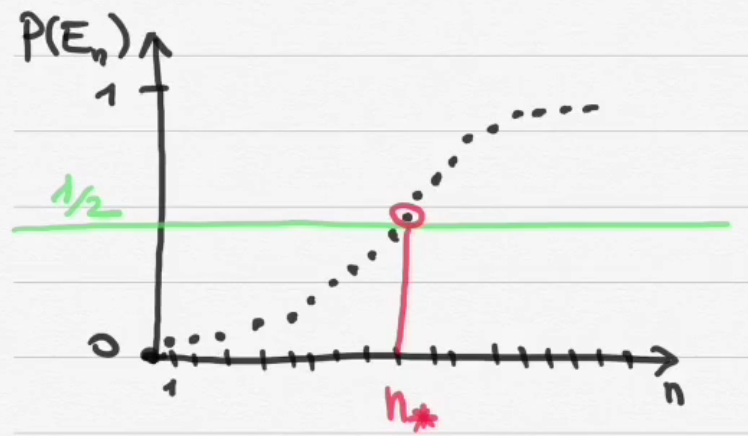
\includegraphics[width = 9cm]{GraficoBirthday.png}
    \caption{Questo è il grafico che permette di vedere che quale è il minimo \(n_*\) da prendere in considerazione}
    \label{fig:BirthdayAttack}
\end{figure}
\chapter{Lezione 5}
\section{Probabilità Condizionata}
\paragraph{Esempio} Urna: 7 palline nere e 3 palline rosse. Estraggo 2 palline. Qual è la probabilità che la seconda pallina estratta sia rossa?\\
La risposta dipende da \textbf{quale pallina ho estratto alla prima estrazione}: la prima estrazione può avere 2 esiti diversi \begin{itemize}
    \item Pallina nera: resteranno \textbf{6 nere} e \textbf{3 rosse}, la probabilità che la seconda pallina sia rossa è \(\frac{1}{3}\)
    \item Pallina rossa: resteranno \textbf{7 nere} e \textbf{2 rosse}, la probabilità che la seconda pallina sia rossa è \(\frac{2}{9}\)
\end{itemize}
quindi la probabilità \textbf{cambia a seconda della scelta} che faccio.\\
Con questo concetto rispondiamo alle affermazioni del tipo: "la probabilità di E sapendo che si è verificato l'evento F".
\section{Definizione Probabilità Condizionata}
Siano \((\Omega, \textit{F}, P)\) uno spazio di probabilità e \(F \in \textit{F}\) un evento tale che \(P(F) > 0\).\\
Allora, per ogni altro evento \(E \in \textit{F}\) è ben definita la quantità \[P(E|F) = \frac{P(E \cap F)}{P(F)}\] Questa è la probabilità condizionata di \textbf{E dato F}.
\paragraph{Osservazione:} Se P(E) e P(F) sono entrambe strettamente positive, allora \[P(E \cap F) = P(E|F)*P(F) = P(F|E)*P(E)\] Questa formula si chiama \textbf{formula di moltiplicazione}, è un trucco per calcolare l'intersezione.
\paragraph{Giustificazione dell'osservazione:} Mettiamoci su uno spazio di probabilità \textbf{uniforme} e supponiamo di avere un'urna fatta in questo modo: \begin{itemize}
    \item Ci sono 8 palline numerate da 1 a 8
    \item Le palline "3", "5" e "8" sono nere
    \item Le restanti palline sono rosse
\end{itemize}
Consideriamo gli eventi: \begin{itemize}
    \item E = "estraggo una pallina con numero pari"
    \item F = "estraggo una pallina rossa"
\end{itemize}
\(P(E) = \frac{1}{2}\). Come cambia la situazione se voglio calcolare \(P(E|F)\)? \[P(E|F) = \frac{P(E \cap F)}{P(F)} = \frac{|E \cap F|}{|\Omega|}*\frac{|\Omega|}{|F|} = \frac{|E \cap F|}{|F|} = \frac{3}{5}\] Questa ultima espressione risponde all'affermazione "casi favorevoli su casi possibili", ma in uno \textbf{spazio di probabilità ridotto}. Quindi si può dire che \textbf{condizionare la scelta riduce lo spazio degli esiti possibili}.
\paragraph{Osservazione} \(P(E|F)\) è \textbf{minore, maggiore o uguale} a \(P(E)\).
\subsection{Teorema}
Sia \(F \in \textit{F}\) un evento con \(P(F) > 0\), allora la mappa \[P(\cdot |F): \textit{F} \xrightarrow{} \mathbb{R}\] \[E \longmapsto P(E|F)\] è una misura di probabilità. Da ciò seguono due conseguenze importanti: \begin{enumerate}
    \item \(P(E^c|F) = 1- P(E|F)\)
    \item \(P(E \cup G|F = P(E|F) + P(G|F) - P(E \cap G|F)\), è la formula di \textbf{inclusione/esclusione}
\end{enumerate}
\paragraph{Attenzione:} Fissato \(E \in \textit{F}\), la mappa di \[P(E|\cdot ): \textit{F} \xrightarrow{} \mathbb{R}\] \[F \longmapsto P(E|F)\] \textbf{non è} una misura di probabilità e quindi \[P(E|F^c) \neq 1 - P(E|F)\]
\section{Formula delle probabilità totali}
\subsection{Teorema}
Siano (\(\Omega, \textit{F}, P\)) uno spazio di probabilità e \(F \in \textit{F}\) un evento tale che \(0 < P(F) < 1\), quindi un evento non impossibile e non certo, allora, per ogni \(E \in \textit{F}\), vale la formula delle probabilità totali: \[P(E) = P(E|F)\cdot P(F) + P(E|F^c)\cdot P(F^c)\] In generale, se ho \(\{F_k\}^n_{k = 1}\) che è una partizione di \(\Omega\) con \(P(F_k) > 0\) per ogni k, vale la formula delle probabilità totali: \[P(E) = \sum^n_{k=1} P(E|F_k)\cdot P(F_k)\]
\paragraph{Dimostrazione:} Dimostriamo il caso generale. Scomponiamo l'evento E sulla partizione \(\{F_k\}^{n}_{k=1}\) ed otteniamo: \[E = \bigcup^{n}_{k=1} (E \cap F_k)\] ovvero una unione disgiunta. Quindi calcoliamo: \[P(E) = P(\bigcup^{n}_{k=1} (E \cap F_k)) = \sum^n_{k=1} P(E \cap F_k)\] che ci porta a \[\sum^n_{k=1} P(E|F_k)\cdot P(F_k)\] c.v.d.
\subsubsection{Esempio}
Urna del primo esempio: 7 palline nere e 3 rosse. Estraggo 2 palline e devo determinare quale è la probabilità che la seconda pallina sia rossa.\\
Definisco gli eventi: \(R_i\) = "l'i-esima pallina estratta è rossa", con i = 1,2 ed ottengo: \[P(R_2) = P(R_2|R_1)\cdot P(R_1) + P(R_2|R_1^c)\cdot P(R_1^c) = \frac{2}{9}\cdot \frac{3}{10} + \frac{1}{3}\cdot \frac{7}{10} = \frac{3}{10}\] dove le frazioni indicano, rispettivamente: \begin{itemize}
    \item La probabilità della seconda pallina estratta dopo aver estratto una rossa (\(\frac{2}{9}\))
    \item La probabilità di estrarre una pallina rossa alla prima estrazione (\(\frac{3}{10}\))
    \item La probabilità di avere una pallina rossa dopo una pallina nera (\(\frac{1}{3}\))
    \item La probabilità di estrarre una pallina nera alla prima estrazione (\(\frac{7}{10}\))
\end{itemize}
\subsection{Esercizio: Tre Urne - Prima parte} \label{EsercizioTreUrne1}
Ho tre urne. \begin{itemize}
    \item Prima urna: 3 palline bianche e 2 nere
    \item Seconda urna: 3 palline bianche e 3 nere
    \item Terza urna: 4 palline bianche e 1 nera
\end{itemize}
Lancio un dado equilibrato: \begin{itemize}
    \item Se esce \textbf{6} estraggo una pallina dalla \textbf{terza urna}
    \item Se esce \textbf{4 o 5} estraggo dalla \textbf{seconda urna}
    \item Negli altri casi estraggo dalla \textbf{prima urna}
\end{itemize}
Quale è la probabilità di estrarre una pallina bianca?
\paragraph{Soluzione} Consideriamo gli eventi \(U_i\) = "peschiamo dall'urna i", con i = 1,2,3 e l'evento B = "peschiamo una pallina bianca". Abbiamo: \begin{itemize}
    \item \(P(U_1) = P(punteggio\ dado \in \{1,2,3\}) = \frac{1}{2}\)
    \item \(P(U_2) = P(punteggio\ dado \in \{4,5\}) = \frac{1}{3}\)
    \item \(P(U_3) = P(punteggio\ dado = 6) = \frac{1}{6}\)
\end{itemize}
Dal testo ci possiamo anche ricavare le probabilità condizionate: \begin{itemize}
    \item \(P(B|U_1) = \frac{3}{5}\)
    \item \(P(B|U_2) = \frac{1}{2}\)
    \item \(P(B|U_3) = \frac{4}{5}\)
\end{itemize}
Quindi, per la formula delle probabilità totali otteniamo: \[P(B) = P(B|U_1)\cdot P(U_1) + P(B|U_2)\cdot P(U_2) + P(B|U_3)\cdot P(U_3)\] che equivale a \[\frac{3}{5}\cdot \frac{1}{2} + \frac{1}{2}\cdot \frac{1}{3} + \frac{4}{5}\cdot \frac{1}{6} = \frac{18}{30} = \frac{3}{5}\]
\subsection{Formula di Bayes}
Questa formula serve per stimare le probabilità a posteriori, quindi a "rovesciare" il condizionamento. Questo avviene da
\[P(F_k|E) = \frac{P(F_k \cap E)}{P(E)}\cdot \frac{P(F_k)}{P(F_k)}\] Dati questi elementi posso capire che \[\frac{P(F_k \cap E)}{P(F_k)} = \frac{P(E|F_k)\cdot P(F_k)}{P(E)}\] ed è questa ultima parte (dopo l'uguale) la formula di Bayes.
\subsubsection{Esercizio: Tre Urne - Seconda Parte}
Tenendo le informazioni della sezione \ref{EsercizioTreUrne1}, sapendo che è stata estratta una pallina bianca, quale è la probabilità che sia stata estratta dalla terza urna?
\paragraph{Soluzione} Dobbiamo calcolare \(P(U_3|B)\). Da quanto visto prima sappiamo che \[P(U_3) = \frac{1}{6},\ P(B|U_3) = \frac{4}{5}\ e\ P(B) = \frac{3}{5}\] Per la formula di Bayes, si ha \[P(U_3|B) = \frac{P(B|U_3)\cdot P(U_3)}{P(B)} = \frac{\frac{4}{5}\cdot \frac{1}{6}}{\frac{3}{5}} = \frac{2}{9}\]
\subsection{Esercizi}
\begin{enumerate}
    \item Lungo un canale di trasmissione sono spediti dati in formato {0,1}. Il canale è disturbato e a volte capita che si trasmetta uno 0 e si riceva un 1 e vicenversa. Si stima che: \begin{itemize}
        \item Se si trasmette uno 0, viene ricevuto correttamente con probabilità 0.95
        \item Se si trasmette un 1, viene ricevuto correttamente con probabilità 0.75
        \item Si sa inoltre che il 70\% dei segnali trasmessi sono 0.
    \end{itemize}
    Viene spedito un segnale lungo il canale, calcolare la probabilità che:
    \begin{itemize}
        \item [a)] Venga ricevuto uno 0
        \item [b)] Si verifichi un errore di trasmissione
        \item [c)] Il segnale spedito fosse uno 0, sapendo che è stato ricevuto uno 0.
    \end{itemize}
    \paragraph{Soluzione} Definiamo gli eventi: \begin{itemize}
        \item \(T_i\) = "Trasmetto il segnale i", con \(i \in \{0, 1\}\)
        \item \(R_i\) = "Ricevo il segnale i", con \(i \in \{0, 1\}\)
    \end{itemize}
    Dal testo ricaviamo che: \[P(R_0|T_0) = 0.95,\ P(R_1|T_1) = 0.75\ e\ P(T_0) = 0.7\] 
    \begin{itemize}
        \item [a)] Dobbiamo calcolare la probabilità di \(P(R_0)\). Uso la formula delle probabilità totali: \[P(R_0) = P(R_0|T_0)\cdot P(T_0) + P(R_0|T_1)\cdot P(T_1)\] Si ha: \begin{itemize}
            \item \(P(R_0|T_1) = P(R_1^c|T_1) = 1 - P(R_1|T_1) = 1 - 0.75 = 0.25\)
            \item \(P(T_1) = P(T_0^c) = 1 - P(T_0) = 1 - 0.7 = 0.3\)
        \end{itemize}
        Sostituisco ed ottengo: \[(0.95\cdot 0.7) + (0.25 \cdot 0.3) = 0.74\]
        \item [b)] Sia E l'evento "Si verifica un errore di trasmissione". \[E = (T_0 \cap R_1) \cup (T_1 \cap R_0)\] Questa è una unione disgiunta, quindi ottengo: \[P(E) = P(T_0 \cap R_1) + P(T_1 \cap R_0) = P(R_1|T_0)\cdot P(T_0) + P(R_0|T_1)\cdot P(T_1)\]
        Si ha : \begin{itemize}
            \item \(P(R_1|T_0 = P(R_0^c|T_0) = 1 - P(R_0|T_0) = 1 - 0.95 = 0.05\)
            \item \(P(R_0|T_1 = P(R_1^c|T_1) = 1 - P(R_1|T_1) = 1 - 0.75 = 0.25\)
        \end{itemize}
        Infine ottengo che \[P(E) = (0.05)\cdot (0.7) + (0.25)\cdot (0.3) = 0.11\]
        \item [c)] Dobbiamo calcolare \(P(T_0|R_0)\). E' una probabilità \textbf{a posteriori}, quindi si usa la formula di Bayes e otteniamo: \[P(T_0|R_0) = \frac{P(R_0|T_0)\cdot P(T_0)}{P(R_0)}\] \[= \frac{(0.95) \cdot (0.7)}{0.74} = 0.9\] 
    \end{itemize}
    \item Siano A,B eventi tali che P(A) = \(\frac{1}{4}\) e \(P(A|B) = P(B|A) = \frac{1}{2}\). Si dica, giustificando, se è vero o falso che: \begin{itemize}
        \item [a)] A e B sono incompatibili
        \item [b)] \(P(A \cap B) = P(A)\cdot P(B)\)
        \item [c)] \(P(A \cap B) > P(A) \cdot P(B)\)
    \end{itemize}
    \paragraph{Soluzione}\begin{itemize}
        \item [a)] \(P(A \cap B) = P(B|A) \cdot P(A) = \frac{1}{8}\). Se A,B fossero incompatibili, si avrebbe \(A \cap B = \varnothing\) e quindi \(P(A \cap B) = 0\). \textbf{FALSO}.
        \item [b)] \(P(A \cap B) = P(A)\cdot P(B)\). Si ha che: \[P(A \cap B) = P(A|B)\cdot P(B)\]. Quindi posso semplificare per P(B) ed otterrei che \[P(A|B) = P(A) \xrightarrow{} \frac{1}{2} = \frac{1}{4}\] il che è \textbf{ASSURDO}. Quindi b) è \textbf{FALSO}.
        \item [c)] Dato \(P(A \cap B) > P(A) \cdot P(B)\), abbiamo, dopo la moltiplicazione per P(B) \[P(A|B) \cdot P(B) > P(A) \cdot P(B) = P(A \cap B) > P(A) \cdot P(B)\] e poichè se P(B) non fosse strettamente positivo, \(P(A|B)\) non esisterebbe nemmeno, concludiamo che c) è \textbf{VERO}.
    \end{itemize}
\end{enumerate}
\chapter{Lezione 6}
\section{Eventi Indipendenti}
\subsection{Indipendenza di due eventi}
Sia \((\Omega, \textit{F}, P)\) spazio di probabilità. Gli eventi \(E, F \in \textit{F}\) si dicono indipendenti se \[P(E \cap F) = P(E) \cdot P(F)\] e si scrive \[E \indep F\ o\ \{E, F\}\ indipendente\]
\paragraph{Attenzione} Indipendenza è \textbf{diverso da} incompatibilità. \begin{itemize}
    \item Indipendenza è una nozione \textbf{probabilistica}, dipende da E,F e dalla misura P.
    \item Incompatibilità è una nozione \textbf{insiemistica}.
\end{itemize}
In particolare, se E,F \(\in \textit{F}\) di probabilità strettamente positiva sono incompatibili, allora \textbf{non possono essere indipendenti}. Infatti, essendo incompatibili, significa che se uno si verifica l'altro \textbf{non può certamente verificarsi}, quindi c'è una \textbf{forte dipendenza} tra i due eventi.
\paragraph{Esempio (banale)}
Qualunque sia \(E \in \textit{F}\), allora \(E \indep \varnothing\ e\ E \indep \Omega\). Infatti, si ha \begin{itemize}
    \item \(P(E \cap \varnothing) = P(\varnothing) = 0 = P(\varnothing) \cdot P(E)\)
    \item \(P(E \cap \Omega) = P(E) = P(E) \cdot P(\Omega)\) dove \(P(\Omega) = 1\)
\end{itemize}
\paragraph{Esempi}
\begin{enumerate}
    \item Lanciamo una moneta e un dado. Lo spazio campionario naturale è \[\Omega = \{(a,i): a \in \{T,C\}, i \in \{1,...,6\}\}\] con la misura uniforme.\\
    Osserviamo che \(|\Omega| = 2\cdot 6 = 12\). Gli eventi: \begin{itemize}
        \item E = "Esce testa"
        \item F = "Esce 4"
    \end{itemize}
    sono indipendenti. Infatti, se calcoliamo \[P(E) = P(\{(T,i): i \in \{1,...,6\}\}) = \frac{1}{2}\] \[P(F) = P(\{(a, 4): a \in \{T,C\}\}) = \frac{1}{6}\] 
    \[P(E \cap F) = P(\{(T,4)\}) = \frac{1}{12}\] otteniamo che \(\frac{1}{12} = P(E \cap F) = P(E)\cdot P(F) = \frac{1}{2}\cdot \frac{1}{6}\)
    Questo ci permette di dire che gli eventi sono indipendenti.
    \item Lanciamo un dado due volte. Lo spazio campionario naturale sarà \[\Omega = \{(i,j): i,j \in \{1,...,6\}\}\] con la misura di probabilità \textbf{uniforme}, quindi tutti gli esiti sono equiprobabili.\\
    Osserviamo che \(|\Omega| = 6 \cdot 6 = 36\). Gli eventi:
    \begin{itemize}
        \item E = "La prima faccia è 4"
        \item F = "La somma dei due punteggi è 9" 
    \end{itemize}
    \textbf{non sono indipendenti}.
    \[P(E) = P(\{(4,j): j \in \{1,...,6\}\}) = \frac{1}{6}\]
    \[P(F) = P(\{(3,6), (4,5), (5,4), (6,3)\}) = \frac{1}{9}\]
    \[P(E \cap F) = P(\{(4,5)\}) = \frac{1}{36}\] poichè è solo una la coppia che rispetta la condizione.\\
    Otteniamo \(\frac{1}{36} = P(E \cap F) \neq P(E)\cdot P(F) = \frac{1}{6} \cdot \frac{1}{9} = \frac{1}{54}\), quindi gli eventi \textbf{non sono indipendenti}.\\
    Se invece prendessimo l'evento G = "la somma dei punteggi è 7 " e sostituissimo F con G, gli eventi E e G sarebbero indipendenti.
\end{enumerate}
\section{Conseguenze elementari dell'indipendenza}
\paragraph{Proposizione 1}Siano E,F \(\in \textit{F}\) con \(P(E) > 0\ e\ P(F) > 0\). Allora le seguenti affermazioni:
    \begin{itemize}
        \item [(i)] \(E \indep F\)
        \item [(ii)] \(P(E|F) = P(E)\)
        \item [(iii)] \(P(F|E) = P(F)\)
    \end{itemize}
    sono \textbf{equivalenti}.
\subsection{Dimostrazione} \begin{itemize}
    \item [(i) \(\xrightarrow{} (ii)\)] \(E \indep F \xrightarrow{implica} P(E \cap F) = P(E)\cdot P(F)\) \[P(E \cap F) = P(E|F) \cdot P(F)\] quindi posso semplificare i \(P(F)\) ed ottengo ciò che volevo dimostrare, ossia \[P(E|F) = P(E)\]
    \item [(ii) \(\xrightarrow{} (iii)\)] \(P(E|F) = P(E) \xrightarrow{(Bayes)} \frac{P(F|E)\cdot P(E)}{P(F)} = P(E)\) semplifico per P(E) e moltiplico per P(F), ottenendo \[P(F|E) = P(F)\]
    \item [(iii) \(\xrightarrow{} (i)\)] \(P(F|E) = P(F) \xrightarrow{implica} \frac{P(E \cap F)}{P(E)} = P(F)\) moltiplico per P(E) ed ottengo \[P(E \cap F) = P(F) \cdot P(E) \xrightarrow{ci\ porta\ a} E \indep F\] c.v.d
\end{itemize}
\subsection{Proposizione 2} Abbiamo \textbf{equivalenza} tra le seguenti istanze:
\begin{itemize}
    \item [(i)] \(E \indep F\)
    \item [(ii)] \(E^c \indep F\)
    \item [(iii)] \(E^c \indep F^c\)
    \item [(iv)] \(E \indep F^c\)
\end{itemize}
\paragraph{Dimostrazione} Abbiamo anche qui una catena di implicazioni: \begin{itemize}
    \item [(i) \(\xrightarrow{} (ii)\)] Dobbiamo mostrare che \(P(E^c \cap F) = P(E^c) \cdot P(F)\). \\
    Si ha \(E^c \cap F = F \backslash (E \cap F)\) ed inoltre si ha che \(E \cap F \subseteq F\).\\
    Quindi \(P(E^c \cap F) = P(F) - P(E \cap F)\). Usiamo l'ipotesi (i), quindi otteniamo: \[P(E^c \cap F) = P(F) - P(E) \cdot P(F) = P(F)\cdot (1-P(E))\] ed \((1-P(E)) = P(E^c)\), quindi \[P(E^c \cap F) = P(E^c)\cdot P(F)\]
    Per concludere si deve dimostrare che \((ii) \xrightarrow{}(iii)\xrightarrow{}(iv)\xrightarrow{}(i)\).
\end{itemize}
\section{Indipendenza di Tre Eventi}
Gli eventi \(E_1, E_2, E_3\) sono indipendenti se le seguenti due condizioni sono \textbf{entrambe} soddisfatte: \begin{enumerate}
    \item \(E_1 \indep E_2, E_1 \indep E_3, E_2 \indep E_3\)
    \item \(P(E_1 \cap E_2 \cap E_3) = P(E_1)\cdot P(E_2) \cdot P(E_3)\)
\end{enumerate}
\paragraph{Osservazione} Le due condizioni \textbf{non sono rindondanti}, sono infatti logicamente \textbf{indipendenti} e necessarie.
\subsection{Esempi}
\begin{enumerate}
    \item Lancio due volte una moneta. Considero gli eventi: \begin{itemize}
        \item A = "al primo lancio ottengo testa"
        \item B = "al secondo lancio ottengo testa"
        \item C = "nei due lanci ottengo due facce uguali"
    \end{itemize}
    Mostriamo che gli eventi sono a 2 a 2 indipendenti, ovvero che \textbf{vale la prima condizione} ma la seconda non è soddisfatta:
    \paragraph{Soluzione} Lo spazio campionario \(\Omega = \{(l_1, l_2): l_1,l_2 \in \{T,C\}\}\) con \(|\Omega| = 2\cdot 2 = 4\)
    \begin{itemize}
        \item Evento A: \(P(A) = P(\{(T,l_2): l_2 \in \{T,C\}\}) = \frac{1}{2}\)
        \item Evento B: \(P(B) = P(\{(l_1, T): l_1 \in \{T,C\}\}) = \frac{1}{2}\)
        \item Evento C: \(P(C) = P(\{(T, T), (C,C)\}) = \frac{1}{2}\)
    \end{itemize}
    Inoltre si ha: \[P(A \cap B) = P(A \cap C) = P(B \cap C) = P(\{(T,T)\} = \frac{1}{4}\]
    Si vede facilmente che le coppie \{A,B\}, \{A,C\} e \{B,C\} sono indipendenti.\\
    Per esempio prendiamo: \[\frac{1}{4} = P(A \cap B) = P(A) \cdot P(B) = \frac{1}{2}\cdot \frac{1}{2}\] le altre sono analoghe.
    Mostriamo ora che \[P(A \cap B \cap C) \neq P(A)\cdot P(B)\cdot P(C)\]
    \begin{itemize}
        \item \(P(A)\cdot P(B)\cdot P(C) = \frac{1}{8}\)
        \item \(P(A \cap B \cap C) = P(\{(T,T)\}) = \frac{1}{4}\)
    \end{itemize}
    \item Lancio due volte un dado. Considero gli eventi: \begin{itemize}
        \item A = "Il punteggio del primo lancio \(\in \{1,2,3\}\)"
        \item B = "Il punteggio del primo lancio \(\in \{3,4,5\}\)
        \item C = "La somma dei due punteggi è uguale a 9"
    \end{itemize}
    \paragraph{Soluzione} Mostriamo che: \begin{itemize}
        \item \(P(A\cap B \cap C) = P(A)\cdot P(B)\cdot P(C)\)
        \item Gli eventi \textbf{non sono indipendenti} a 2 a 2.
    \end{itemize}
    Lo spazio campionario è \[\Omega = \{(d_1, d_2): d_1,d_2 \in \{1,...,6\}\} \xrightarrow{} |\Omega| = 6\cdot 6 = 36\]
    Calcoliamo: \begin{itemize}
        \item \(P(A) = P(\{(d_1,d_2): d_1 \in \{1,2,3\}, d_2 \in \{1,...,6\}\}) = \frac{3\cdot 6}{36} = \frac{1}{2}\)
        \item \(P(A) = P(\{(d_1,d_2): d_1 \in \{3,4,5\}, d_2 \in \{1,...,6\}\}) = \frac{3\cdot 6}{36} = \frac{1}{2}\)
        \item \(P(C) = P(\{(3,6), (4,5), (5,4), (6,3)\}) = \frac{1}{9}\)
    \end{itemize}
    Inoltre: \[P(A\cap B\cap C) = P(\{(3,6)\} = \frac{1}{36}\]
    Quindi \[P(A\cap B\cap C) = \frac{1}{36} = P(A)\cdot P(B)\cdot P(C) = \frac{1}{2}\cdot \frac{1}{2}\cdot \frac{1}{9} = \frac{1}{36}\] 
    Consideriamo ora \{A,C\} e mostriamo che non sono indipendenti. Sappiamo già che: \[P(A)\cdot P(C) = \frac{1}{2}\cdot \frac{1}{9} = \frac{1}{18}\]
    Calcoliamo \[P(A\cap C) = P(\{3,6\}) = \frac{1}{36}\]
    Si può facilmente vedere che \[\frac{1}{18} \neq \frac{1}{36}\]
    quindi gli eventi \textbf{non sono a due a due indipendenti}. Si può procedere in modo analogo per le altre coppie, ma il risultato è lo stesso: basta che solo una coppia non soddisfi la condizione e anche le altre non la soddisferanno.
\end{enumerate}
\subsection{In generale}
La famiglia di \(\{E_1,...,E_n\}\) di eventi è indipendente se \textbf{per ogni r} (\(2 \leq r \leq n\)) e per \textbf{ogni possibile scelta di r eventi distinti} degli n eventi della famiglia, la probabilità dell'intersezione degli r eventi scelti è \textbf{pari al prodotto delle loro probabilità}.\\
Devo quindi dimostrare la \textbf{proprietà di fattorizzazione} per ogni coppia, terna, quaterna, ecc. di eventi. Devo considerare \textbf{tutte le possibili sottofamiglie}.
\paragraph{Osservazione} Se \(\{E_1,...,E_n\}\) è una famiglia di eventi indipendenti, quando sostituisco qualche \(E_i\) (non importa quanti e quali) con \(E_i^c\) ottengo ancora una famiglia di eventi \textbf{indipendenti}.\\
La famiglia \textbf{numerabile} di eventi \(\{E_1,E_2,...\}\) è indipendente se ogni sottofamiglia finita lo è.

\chapter{Lezione 7}
\section{Variabili Aleatorie Discrete}
Sia (\(\Omega, \Pn(\Omega), P\)) uno spazio di probabilità discreto. Ogni mappa: \[X: \Omega \xrightarrow{} \mathbb{R}\] è detta \textbf{variabile aleatoria} (o casuale) discreta su \(\mathbb{R}\).\\
Nella mappa X, \textbf{ad ogni esito viene associato un numero}.
\begin{figure}[hb]
    \centering
    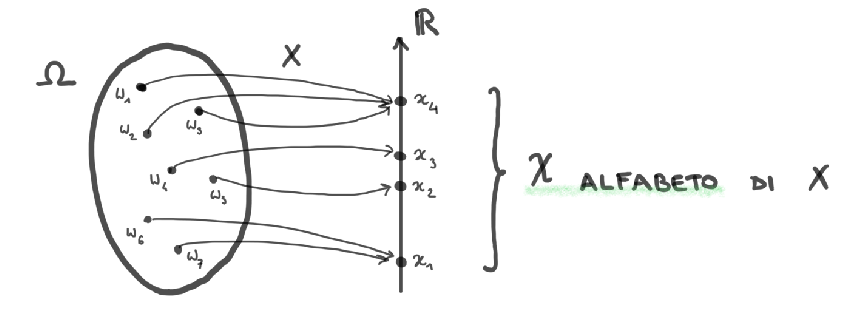
\includegraphics[width = 10cm]{AlfabetoX.png}
    \caption{Vediamo qui l'Alfabeto di X, che è l'immagine di X}
    \label{fig:AlfabetoX}
\end{figure}
Abbiamo che \[\textit{X} = X(\Omega) = \{x \in \mathbb{R}:\ X(\omega) = x\ per\ qualche\ \omega \in \Omega\}\]
\paragraph{Importante!} \textit{X} è \textbf{discreto} ed ho che \[|\textit{X}| \leq |\Omega| \leq |\mathbb{N}|\]
\subsection{Esempi}\begin{enumerate}
    \item Sia (\(\Omega,\Pn(\Omega), P\)) uno spazio di probabilità discreto. Sia E \(\in \Pn(\Omega)\) un qualsiasi evento. Possiamo definire la variabile aleatoria \(\mathds{1}_E (\omega): \Omega \xrightarrow{} \mathbb{R}\) definita come: \[
    \mathds{1}_E (\omega) = \begin{cases}
    1, & \text{se }\omega \in E\\
    0, & \text{altrimenti}
    \end{cases}
    \]
    Questa variabile si chiama \textbf{indicatrice} ed ha alfabeto \{0,1\}.
    \item Sia ora \(\Omega = \{(d_1,d_2): d_1,d_2 \in \{1,...,6\}\}\) lo spazio campionario relativo al lancio di una coppia di dadi, dove \(d_i\) indica il punteggio dell'i-esimo dado, ed i = 1,2.\\
    Vediamo qualche variabile aleatoria che si può creare.
    \begin{itemize}
        \item \(\omega = (d_1,d_2) \longmapsto X_1(\omega) = d_1\) \\ 
        Mappo gli eventi verso la variabile aleatoria \(X_1\) e questo mi dice di considerare solo il lancio del valore \(d_1\). L'alfabeto sarà \(X_1 = \{1,...,6\}\). Il discorso sulla mappatura vale anche per i prossimi esempi.
        \item \(\omega = (d_1,d_2) \longmapsto X_2(\omega) = d_2\) con alfabeto \(X_2 = \{1,...,6\}\)
        \item \(\omega = (d_1,d_2) \longmapsto X_3(\omega) = min \{d_1,d_2\}\) con alfabeto \(X_3 = \{1,...,6\}\)
        \item \(\omega = (d_1,d_2) \longmapsto X_4(\omega) = max \{d_1,d_2\}\) con alfabeto \(X_4 = \{1,...,6\}\)
        \item \(\omega = (d_1,d_2) \longmapsto X_5(\omega) = d_1 + d_2\) con alfabeto \(X_5 = \{2,3,...,12\}\)
    \end{itemize}
\end{enumerate}
\paragraph{Osservazione} Se vengono definite sullo stesso spazio di probabilità, diverse variabili aleatorie possono essere \textbf{combinate} attraverso \textbf{operazioni}, come ad esempio \[X+Y, X-Y, X\cdot Y, X/Y, min \{X,Y\}, max \{X, Y\}\] queste sono ancora variabili aleatorie, come nell'esempio 2, in cui avevamo \(X_3, X_4 \text{ e }X_5\).
\section{Misura di probabilità indotta}
Poichè \textit{X} è un insieme discreto, basta assegnare una probabilità \(P^X\) ad \textbf{ogni singoletto} di \textit{X}, compatibile con la probabilità P di (\(\Omega, \Pn(\Omega), P\)) dove X è definita.
\subsection{Definizione Probabilità Indotta} La definizione è questa: \[P^X(x_k) = P(X^{-1}(x_k)) \forall x_k \in \textit{X}\] che si può anche scrivere come: \[P^X(x_k) = P(X = x_k) \forall x_k \in \textit{X}\]
Cosa significa? Significa che la probabilità totale dei valori che fanno verificare \(x_k\) è \textbf{uguale} alla probabilità che si verifichi \(x_k\) dell'alfabeto.\\
Ciascuno dei valori dell'alfabeto si osserverà se \textbf{qualcuno degli esiti mappati in questo valore si verifica}.
\subsection{Lemma e Dimostrazione} \(P^X\) è una misura di probabilità.
\paragraph{Dimostrazione} Poichè \textit{X} è discreto, basta verificare: \begin{enumerate}
    \item \(P^X (x_k) \geq 0\) \(\forall x \in \textit{X}\)
    \item \(\sum_{x_k \in \textit{X}}P^X (x_k) = 1\)
\end{enumerate}
\paragraph{Verifico} \begin{enumerate}
    \item \(P^X(x_k) = P(X^{-1}(x_k))\) ma P è misura di probabilità e quindi positiva
    \item Osserviamo il fatto che X sia una funzione: ciò implica che la funzione delle anti-immagini (ovvero gli esiti che poi vengono mappati nell'alfabeto) \[\{X^{-1}(X_k)\}_{x_k \in \textit{X}}\] sia una \textbf{partizione} di \(\Omega\), cioè: \begin{itemize}
        \item \(X^{-1}(x_k) \cap X^{-1}(x_j) = \varnothing,\ \forall k \neq j\)
        \item \(\bigcup_{x_k \in \textit{X}} X^{-1}(x_k) = \Omega\)
    \end{itemize}
    Quindi otteniamo che: \[\sum_{x_k \in \textit{X}}P^X (x_k) = \sum_{x_k \in \textit{X}}P(X^{-1}(x_k))\] \[= P(\bigcup_{x_k \in \textit{X}} X^{-1} (x_k))\] \[= P(\Omega) = 1\] come volevasi dimostrare.
    \begin{figure}[hb]
        \centering
        \includegraphics[width = 12cm]{NuvoleProbabilità.png}
        \caption{In questa figura vediamo chiaramente che le nuvole di probabilità sono distinte e disgiunte e si può vedere chiaramente ciò che è stato appena dimostrato.}
        \label{fig:NuvoleProbabilita}
    \end{figure}
\end{enumerate}
\clearpage
\section{Esempi e descrizione probabilistica}
\begin{enumerate}
    \item Ritorniamo all'esempio del lancio di 2 dadi, e consideriamo la variabile aleatoria \(X_1: \Omega \longmapsto \mathbb{R} \text{ con } (d_1, d_2) \mapsto d_1\)\\
    Come assegniamo una probabilità sull'alfabeto \(\textit{X}_1 = \{1, ..., 6\}\)? Vediamolo con una figura:
    \begin{figure}[hb]
        \centering
        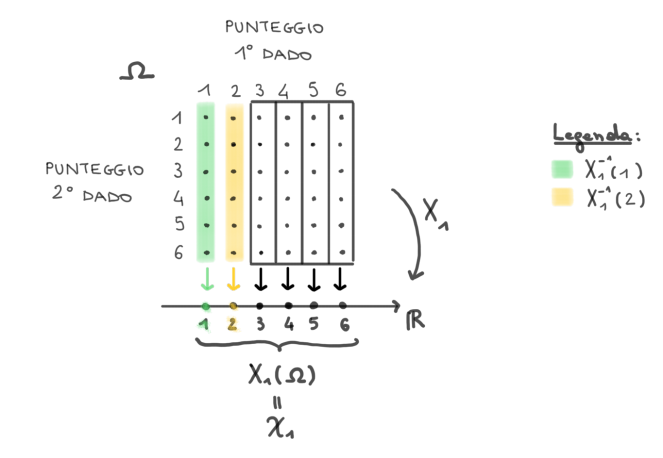
\includegraphics[width = 11cm]{VariabileAleatoriaLancio2dadi.PNG}
        \caption{Vediamo qui che ogni lancio del primo dado, come lo abbiamo definito prima, porta alla rappresentazione del numero reale, e l'insieme dei valori dati da \(d_1\) mi dà l'alfabeto \(\textit{X}_1\) }
        \label{fig:VariabileAleatoriaLancioDadi}
    \end{figure}
    La probabilità delle anti-immagini è:
    \[P^{X_1}(1 \in X_1) = P(X = 1) = P(X_1^{-1}(1))\] \[= P(\{(1,1), (1,2), ..., (1,6)\}) = \frac{1}{6}\]\\
    \[P^{X_1}(2 \in X_1) = P(X = 2) = P(X_1^{-1}(2))\] \[= P(\{(2,1), (2,2), ..., (2,6)\}) = \frac{1}{6}\] 
    Analogamente possiamo trovare \[P^{X_1}(3) = P^{X_1}(4) = P^{X_1}(5) = P^{X_1}(6) = \frac{1}{6}\]
    \clearpage
    \item Sempre dall'esempio del lancio dei 2 dadi: consideriamo \[X_3: \Omega \xrightarrow{} \mathbb{R}\] \[(d_1,d_2) \mapsto min\{d_1,d_2\}\]
    Come assegnamo una probabilità su \(X_3 = \{1,...,6\}\)?
    \begin{figure}[hb]
        \centering
        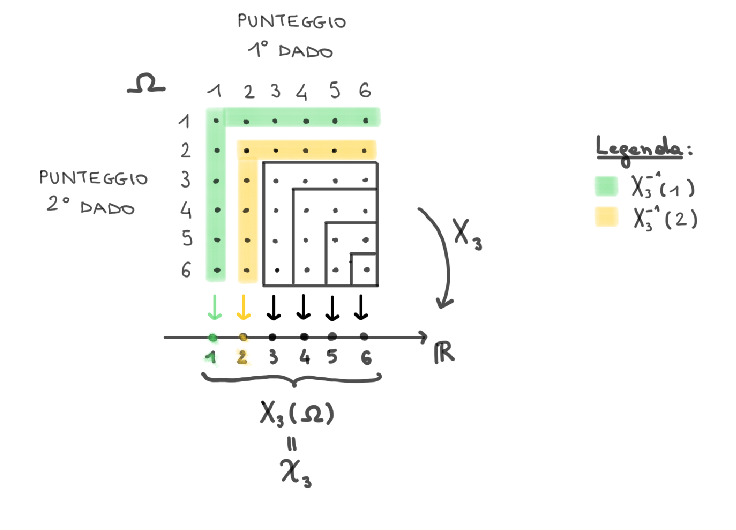
\includegraphics[width = 10cm]{PunteggioDadi2-Lez7.png}
        \caption{}
        \label{fig:Esempio2Lez7}
    \end{figure}
    \[P^{X_3}(1) = P(X_3^{-1}(1)) = P(X = 1) = P(\text{ parte verde }) = \frac{11}{36}\]
    \[P^{X_3}(2) = P(X_3^{-1}(2)) = P(2) = P(\text{ parte gialla }) = \frac{1}{4}\]
    e così via per tutti gli elementi dell'alfabeto \(X_3\)
\end{enumerate}
\subsection{Descrizione Probabilistica della variabile aleatoria}
Se X è una variabile aleatoria discreta, per definirla probabilisticamente utilizziamo questa descrizione:
\begin{itemize}
    \item Abbiamo \textit{X} alfabeto \textbf{unito} a 
    \item \(p_x: \textit{X} \xrightarrow{}[0,1]\\
    x_k \longmapsto p_x(x_k) = P(X = x_k)\) dove esistono due proprietà: \begin{enumerate}
        \item \(p_x(x_k) \geq 0, \forall x_k \in \textit{X}\)
        \item \(\sum_{x_k \in \textit{X}} p_x(x_k) = 1\)
    \end{enumerate}
\end{itemize}
Identifichiamo \(p_x\) come \textbf{densità discreta di probabilità} (o \textbf{legge}) della variabile aleatoria X.
\subsubsection{Esempio}
Sia X una var. aleatoria discreta con alfabeto \(\textit{X}=\{0, \sqrt{2}, \pi\}\) e densità discreta \begin{itemize}
    \item \(p_x(0) = \frac{2}{3}\)
    \item \(p_x(\sqrt{2}) = p_x(\pi) = \frac{1}{6}\)
\end{itemize}
Calcoliamo \(P(1 < X < 4)\). Abbiamo:  
\begin{align}
P(1 < X < 4) & = P(X \in \{\sqrt{2}, \pi\})\\
& = P(\{X = \sqrt{2}\} \cup \{X = \pi\})\\
& = P(X = \sqrt{2} + P(X = \pi)\\
& = \frac{1}{3}    
\end{align}
\chapter{Lezione 8}
Ricapitolando possiamo definire una variabile aleatoria in due modi: \begin{enumerate}
    \item Come funzione \(X: \Omega \xrightarrow{} \mathbb{R}\) di cui si determinano alfabeto \textit{X} e misura di probabilità indotta \(P^x(x_k) = P(X^{-1}(x_k))\), per ogni \(x_k \in \textit{X}\), da cui si deduce la densità \(p_x(x_k) = P^{x}(x_k)\), per ogni \(x_k \in \textit{X}\), che soddisfa positività e normalizzazione.
    \item Si danno direttamente alfabeto \textit{X} e densità \(p_x(\cdot)\) che soddisfa positività e normalizzazione.
\end{enumerate}
\section{Funzione di una variabile aleatoria}
\(
\begin{rcases}
X:\Omega \xrightarrow{} \mathbb{R}, & \text{variabile aleatoria}\\
g:\mathbb{R} \xrightarrow{} \mathbb{R}, & \text{funzione}
\end{rcases}
\) Y = g\(oX:\Omega \xrightarrow{} \mathbb{R}\)
 variabile aleatoria\\
Caratterizziamo Y. L'alfabeto è \textit{Y} = g(\textit{X}) e la densità discreta:
\[p_Y(y_l) = P(Y=y_l) = \sum_{x:g(x_k) = y_l} p_x(x_k) \text{, per ogni }y_l \in \textit{Y}\]
\subsubsection{Esempio}
Sia X una v.al. con alfabeto \textit{X} = \{-1,1,3\} e densità discreta \(p_x(-1) = p_x(3) = \frac{1}{4}\) e \(p_x(1) = \frac{1}{2}\).\\
Caratterizziamo la v.al. Y=\(X^2\): se \begin{itemize}
    \item g: \(\mathbb{R} \xrightarrow{} \mathbb{R}\)
    \item g: x \(\longmapsto x^2\)
\end{itemize}
abbiamo Y = g(X).\\
Alfabeto: \textit{Y} = g(\textit{X}) = \{1,9\}\\
Densità: \begin{align}
    p_y(1) & = P(\{X = -1\} \cup \{X = 1\})\\
    & = p_x(-1) + p_x(1) = \frac{1}{4}+\frac{1}{2} = \frac{3}{4}\\
   & P_y(9) = P(X=3) = p_x(3) = \frac{1}{4}
\end{align}
\subsection{Esercizi}
\begin{enumerate}
    \item Lancio una moneta e un dado. Se i risultati che ottengo hanno la stessa iniziale vinco 1 euro, altrimenti perdo 50 centesimi.\\ 
    Sia X la variabile aleatoria che descrive la vincita/perdita. Determinare alfabeto e densità discreta di X.
    \begin{itemize}
        \item \textbf{Soluzione}: Alfabeto: \textit{X} = \(\{\frac{-1}{2}, 1\}\), corrispondono a perdita e vincita.\\
    \item Densità discreta: Uno spazio campionario per il nostro gioco è \[\Omega = \{(a,i): a \in \{T,C\}, i \in \{1,...,6\}\}\]
    Si ha \(|\Omega| = 2 \cdot 6 = 12\). Calcoliamo la probabilità indotta, che prendiamo come densità di X.
    \begin{align}
        p_x(1) = P(X = 1) & = P(\text{i risultati hanno la stessa iniziale})\\
        & = P(\{(T,3), (C,5)\} = \frac{1}{6}\\
        & p_x(- \frac{1}{2} = 1 - p_x(1) = \frac{5}{6}
    \end{align}
    \end{itemize}
    \item Estraggo tre carte da un mazzo di carte da poker. Vinco 1 euro per ogni carta di picche estratta.\\
    Sia X la variabile aleatori che descrive la vincita. Determinare alfabeto e densità discreta di X.
    \begin{itemize}
        \item \textbf{Soluzione}: Alfabeto: \textit{X} = \{0,1,2,3\}
        \item Densità discreta:
        \begin{align}
            p_x(0) = P(X = 0) & = P (\text{non pesco carte di picche})\\
            & = \frac{\binom{39}{3}}{\binom{52}{3}} = \frac{703}{1700}
        \end{align}
        \begin{align}
            p_x(1) = P(1) & = P (\text{pesco 1 carta di picche})\\
            & = \frac{13 \cdot \binom{39}{2}}{\binom{52}{3}} = \frac{741}{1700}
        \end{align}
        \begin{align}
            p_x(2) = P(2) & = P (\text{pesco 2 carte di picche})\\
            & = \frac{\binom{13}{2} \cdot 39 }{\binom{52}{3}} = \frac{234}{1700}
        \end{align}\\
        \(p_x(3) = 1 - p_x(0) - p_x(1) -p_x(2) = \dfrac{11}{850}\)
    \end{itemize}
\end{enumerate}
\section{Valor Medio (o Atteso)}
Sia X v.al. con alfabeto \textit{X} e densità discreta \(p_x\). Il valor medio di X è il numero reale: 
\[E(x) = \sum_{x_k \in \textit{X}} x_k \cdot p_x(x_k)\]
\paragraph{Osservazione} Se \(|\textit{X}| < \infty\), allora il v.medio è una somma \textbf{finita} ed è \textbf{sempre} ben definito. Se \(|\textit{X}| = +\infty\), allora il v.medio è una serie e \textbf{può non esistere} se la serie \textbf{non converge}.
\subsubsection{Esempi}
\begin{enumerate}
    \item Sia X una v.al. con alfabeto \textit{X} = \(\{-7,0,\pi,4\}\) e densità \(p_x(-7) = \frac{1}{2}\) e \(p_x(0) = p_x(\pi) = p_x(4) = \frac{1}{6}\). Otteniamo:
    \[E(X) = (-7) \cdot \frac{1}{2} + (4+\pi) \cdot \frac{1}{6} \approx -2.31\]
    \item Consideriamo uno spazio di probabilità (\(\Omega, \mathbb{P}(\Omega),P\)) ed un evento \(E \in \mathbb{P}(\Omega)\). Definiamo la v.al.
    \[
    X(\omega) = \mathds{1}_{E}(\omega) = 
    \begin{cases}
    1, & \text{ se } \omega \in E \\
    0, & \text{ se } \omega \notin E \\
    \end{cases}
    \]
    Allora si ha:
    \[E(X) = P(X = 1) = P(\{\omega: X(\omega) = 1\}) = P(E)\]
    \end{enumerate}
\subsection{Significato del Valor Medio}
Indice di centralità \(\Longleftrightarrow\) Baricentro della distribuzione.\\
%figura
abbiamo dei punti \(\{x_1,...,x_n\}\) con masse \(p_x(x_1),...,p_x(x_n)\) e cerchiamo il baricentro \(a \in \mathbb{R}\) della nuvola di punti. Cerchiamo il punto dove la risultante dei momenti è nulla (\textbf{equilibrio}):
\begin{align}
  & \sum_{x_k}(x_k - a) \cdot p_x(x_k) = 0\\
  & \Longleftrightarrow \sum_{x_k} x_k \cdot p_x(x_k) = a\cdot \underbrace{\sum_{x_k}p_x(x_k)}_\text{= 1}\\
  & \Longleftrightarrow a = E(x)
\end{align}
\subsection{Teorema Fondamentale del valor medio}
Sia \(X: \Omega \xrightarrow{} \mathbb{R}\) una v.al. discreta, allora si ha:
\[E(X) = \sum_{\omega \in \Omega} X(\omega)\cdot P(\{\omega\})\]
\subsubsection{Dimostrazione}
Calcoliamo:
    \[E(X) = \sum_{x_k \in \textit{X}} x_k \cdot p_x (x_k)  = \sum_{x_k \in \textit{X}} x_k \cdot P(X^{-1}(x_k))\]\\
    \begin{align}
    \text{(definizione di antiimmagine)} & = \sum_{x_k \in \textit{X}} x_k \cdot P(\underbrace{\{\omega: X(\omega) = x_k\})}_\substack{
    \textbf{Insieme discreto}: \text{ottengo la sua} \\
    \text{probabilità} \\
    \text{sommando le probabilità degli esiti}\\
    \text{che ci appartengono}}\\
    & = \sum_{x_k \in \textit{X}}x_k \cdot \sum_{\omega: X(\omega) = x_k} \cdot P(\{\omega\})\\
    & = \underbrace{\sum_{x_k \in \textit{X}}x_k \cdot \sum_{\omega: X(\omega) = x_k}}_\text{vedi (1) sotto} \cdot X(\omega) \cdot P(\{\omega\})\\
    & = \sum_{\omega \in \Omega} X(\omega) \cdot P(\{\omega\})
    \end{align}
    (1): Le due somme descrivono l'insieme: \[\bigcup_{x_k \in \textit{X}} \{\omega : X(\omega) = x_k\} = \Omega\]
    \[\text{ dove } X(\omega) \longleftrightarrow \{X^{-1}(x_k)\} \text{ (è una partizione)}\]
\chapter{Lezione 9}
\section{Proprietà del Valor Medio}
\subsection{Linearità}
Descriviamo la linearità attraverso due osservazioni: \begin{enumerate}
    \item Sia X una v.al., \(a \in \mathbb{R}\), allora \(E(aX) = aE(X)\). Come lo vedo?\\
    \textit{a}X è la v.al. \(\omega \mapsto aX(\omega)\), allora per il teorema fondamentale otteniamo:
    \begin{align}
        E(aX) & = \sum_{\omega \in \Omega}aX(\omega)P(\{\omega\})\\
        & = a \sum_{\omega \in \Omega} X(\omega) P(\{\omega\}) = aE(X)
    \end{align}
    \item Siano X,Y v.al. definite sullo stesso spazio campionario \(\Omega\). Allora E(X+Y) = E(X) + E(Y). Come lo vedo?\\
    X + Y è la v.al. \(\omega \mapsto X(\omega) + Y(\omega)\), allora per il teorema fondamentale otteniamo:
    \begin{align}
        E(X + Y) & = \sum_{\omega \in \Omega} (X(\omega) + Y(\omega))P(\{\omega\})\\
        & = \sum_{\omega \in \Omega} X(\omega)\cdot P(\{\omega\}) + Y(\omega)\cdot P(\{\omega\})\\
        & = E(X) + E(Y)
    \end{align}
\end{enumerate}
Potevo definire la proprietà 2. con la definizione del valore medio? 
\[E(X+Y) = \sum_{x_k \in \textit{X}} \sum_{y_l \in \textit{Y}} (x_k + y_l) \cdot p_{X+Y}(x_k +y_l)\]
La scrittura \(p_{X+Y}\) avrà senso dalla settimana 8.\\
Mettendo insieme le proprietà 1. e 2. otteniamo: \[E(aX+bY) = aE(X) + bE(Y)\]
\subsection{Positività}
Sia X una v.al. positiva (cioè \textit{X} \(\in \mathbb{R_{+}}\)), allora \(E(X) \geq 0\)
\subsection{Monotonia}
Siano X, Y: \(\Omega \xrightarrow{} \mathbb{R}\) v.al. tali che \(X \geq Y\). Allora si può dire che \[E(X) \geq E(Y)\]
Come lo vedo?\\
\(X \geq Y \Longleftrightarrow X - Y \geq 0\).\\ 
Per la positività si ha che \(E(X-Y) \geq 0\).\\ 
Per la linearità invece si ottiene \(E(X) - E(Y) \geq 0\) da cui concludo la dimostrazione che \(E(X) \geq E(Y)\).
\subsection{Limiti Inferiore e Superiore}
Sia X v.al. con alfabeto \textit{X} e siano \(\underline{x} = inf \textit{X}\) e \(\overline{x} = sup \textit{X}\). Allora si ha: \[\underline{x} \leq E(X) \leq \overline{x}\]
\paragraph{Osservazione:} Se \(b \in \mathbb{R}\) allora E(b) = b.\\
Possiamo vedere \(b \in \mathbb{R}\) come una v.al. \textbf{costante}, cioè:\\
X v.al. con alfabeto \textit{X} = \{b\} e densità discreta \(p_x(b) = 1\) e\(p_x(i) = 0\) \(\forall i \neq b\).\\
Segue dalla definizione di valor medio che E(X) = b.
\subsection{Teorema (valor medio di funzioni di v.al.)}
Siano \(X: \Omega \xrightarrow{} \mathbb{R}\) v.al. e \(g: \mathbb{R} \xrightarrow{} \mathbb{R}\) funzione. Si ha: \[E(g(X)) = \sum_{x_k \in \textit{X}} g(x_k) p_x(x_k)\]
\subsubsection{Esempio}
Sia X v.al. con alfabeto \textit{X}=\{-1,1,3\} e densità discreta \(p_x(3) = p_x(-1) = \frac{1}{4} \text{ e }p_x(1) = \frac{1}{2}\). Sia inoltre \(Y = X^2\). Calcoliamo E(Y).
\begin{itemize}
    \item \textbf{Metodo 1:} Caratterizzo Y (alfabeto + densità) e uso la definizione di valor medio.\\
    Abbiamo \textit{Y} = \{1,9\} e \(p_y(1) = \frac{3}{4} \text{ e } p_y (3) = \frac{1}{4}\).\\
    Quindi \[E(Y) = 1 \cdot \frac{3}{4} + 9 \cdot \frac{1}{4} = 3\]
    \item \textbf{Metodo 2:} Applico direttamente il teorema: 
    \[E(Y) = (-1)^2 \cdot \frac{1}{4} + 1^2 \cdot \frac{1}{2} + 3^2 \cdot \frac{1}{4} = 3\]
\end{itemize}
\subsection{Esercizi}
\begin{enumerate}
    \item Un'urna contiene 8 palline nere e 6 bianche. Si fanno due estrazioni senza reinserimento. Per ogni pallina nera estratta si vince 1 euro. Per ogni pallina bianca estratta si perde 1 euro. Sia X la variabile aleatoria che descrive la vincita/perdita del gioco. Calcolare E(X).
    \paragraph{Soluzione:} Alfabeto: \textit{X} = \{-2, 0, 2\} (corrisponde a: estraggo 2 bianche, estraggo 1 nera e 1 bianca, estraggo 2 nere).\\
    Densità: 
    \begin{align}
      p_x(-2) & = \text{ P(estraggo 2 bianche)}\\
      & = \frac{\binom{6}{2}}{\binom{14}{2}} = \frac{15}{91}
      \end{align}
      \begin{align}
      & p_x(0) = \frac{8\cdot 6}{\binom{14}{2}} = \frac{48}{91}\\
      & p_x(2) = 1 - p_x(0) - p_x(-2) = \frac{4}{13}
      \end{align}
    Media: \(E(X) = (-2) \cdot \frac{15}{91} + 2\cdot \frac{4}{13} = \frac{2}{7} \approx 0.286\)
    \item Due dadi sono truccati in modo che la probabilità di ottenere 6 sia il doppio di quella di ottenere ogni altro punteggio. Qual è la media del punteggio ottenuto lanciando i due dadi?
    \paragraph{Soluzione:} Siano \(X_1 \text{ e } X_2\) le v.al. che corrispondono al punteggio del primo e del secondo dado. Le 2 v.al. hanno lo stesso alfabeto \textit{X}=\{1,...,6\} e la stessa densità discreta che ora determiniamo:\\
    si ha \(p_{xi}(6) = 2p\)\\
    \(p_{xi}(j) = p\) per ogni j = 1,...,5\\
    da cui ricavo \(2p+5p = 1 \Longleftrightarrow p = \frac{1}{7}\).\\
    Quindi la densità è \[p_{xi}(1) = ... = p_{xi} (5) = \frac{1}{7} \text{ e } p_{xi}(6) = \frac{2}{7}\]
    Ora sia \(Y = X_1 + X_2\) la v.al. che corrisponde alla somma dei due punteggi. Abbiamo:
    \begin{align}
        E(Y) & = E(X_1) + E(X_2) \\
        & = (1 + 2 + 3 + 4 + 5) \cdot \frac{1}{7} + 6 \cdot \frac{2}{7} + \frac{15}{7} + \frac{12}{7}\\
        & = \frac{54}{7} \approx 7.7
    \end{align}
    Se i dadi non fossero stati truccati si avrebbe E(Y) = 7.
\end{enumerate}
\subsection{Varianza}
Sia X v.al. con alfabeto \textit{X} e densità discreta \(p_x\). La varianza è il \textbf{numero reale \underline{positivo}}.
\[Var(X) = \sum_{x_{k} \in \textit{X}}(x_k - E(X))^{2} p_x(x_k)\]
\subsubsection{Esempio}
Consideriamo \(X_1 \in \{-1, \frac{1}{4}, \frac{3}{4}\}\) con densità discreta \(p_{x_1} (-1) = p_{x_1} (\frac{1}{4}) = p_{x_1} (\frac{3}{4}) = \frac{1}{3}\) e \(X_2 \in \{-10,10\}\) con densità discreta \(p_{x_2}(-10) = p_{x_2}(10) = \frac{1}{2}\).\\
Abbiamo \(E(X_1) = E(X_2) = 0\), ma
\[Var(X_1) = \frac{1}{3}\cdot[(-1-0)^2 + (\frac{1}{4} - 0)^2 + (\frac{3}{4} - 0)^2] \approx 0.524\]
\[Var(X_2) = \frac{1}{2}\cdot[(-10-0)^2 + (10 - 0)^2] = 100\]
I valori di \(X_2\) sono tanto dispersi, cioè \textbf{lontani dalla media}.
\subsubsection{Proprietà della Varianza}
\begin{enumerate}
    \item Var(X) = \(E[(X-E(X))^2]\) è la media di una funzione della v.al. X; usiamo g(x) = \((x-E(x))^2\)
    \item Var(X) \(\geq 0\) e, in particolare, Var(X) = 0 \(\Longleftrightarrow X \equiv\) costante\\
    Come lo vedo?\\
    \begin{align}
        Var(X) = 0 & \Longleftrightarrow \sum_{x_k \in \textit{X}}(x_k - E(X))^2 \cdot \underbrace{p_x(x_k)}_{> 0} = 0\\
        & \Longleftrightarrow x_k - E(X) = 0, \forall x_k \in \textit{X}\\
        & \Longleftrightarrow x_k = E(X), \forall x_k \in \textit{X}
    \end{align}
    \item Var(aX) = \(a^2\) Var(X), a \(\in \mathbb{R}\)\\
    Come lo vedo?
    \begin{align}
        Var(aX) & = E[(aX - aE(x))^2]\\
       \text{per linearità valor medio } & = E[(aX - aE(x))^2]\\
       \text{per linearità valor medio } & = a^2 E[(X - E(X))^2] = a^2 Var(X)
    \end{align}
    \item Var(X+c) = Var(X), \(c \in \mathbb{R}\)\\
    \paragraph{Osservazione Importante:} 3 e 4 mostrano che la varianza \textbf{NON E' LINEARE!}
    \item Var(X) = \(E(X^2) - E(X)^2\)\\
    Come lo vedo?
    \begin{align}
        Var(X) & = E[(X - E(X))^2]\\
        & = E[X^2 - 2XE(X) + E(X)^2]\\
    (1) & = E(X^2) - E(X)^2
    \end{align}
    (1) Indica che tale risoluzione è data da \(E(X) \in \mathbb{R}\) + linearità del valor medio.
\end{enumerate}
\subsubsection{Esercizio}
L'urna 1 ha composizione: 1 pallina dorata, 4 palline verdi, 15 palline bianche. L'urna 2 invece contiene: 4 palline verdi e 25 palline bianche. Una pallina a caso viene spostata dall'urna 1 all'urna 2, quindi mi viene chiesto di estrarre una pallina dall'urna 2.\\
Se estraggo la pallina dorata vinco 50 euro, se estraggo una pallina verde perdo 1 euro, altrimenti non vinco e non perdo.\\
Sia X la v.al. che corrisponde alla vincita/perdita. Si calcoli la varianza di X.
\paragraph{Soluzione:} Alfabeto \textit{X} = \{-1, 0, 50\}\\
Densità discreta. Considero gli eventi \(T_i = \text{ "trasferisco una pallina i" con } i = O, V, B\), dove O sta per Oro, V per Verde e B per bianca,\\
ed \(E_i = \text{ "estraggo una pallina i" con } i = O,V,B\).\\
Otteniamo:
\begin{align}
    P(X=-1) = P(E_V) = P(E_V | T_B)\cdot P(T_B) & + P(E_V | T_V) \cdot P(T_V)\\ 
    & + P(E_V | T_O) \cdot P(T_O)
    \end{align}
    \[= \frac{4}{30}\cdot \frac{15}{20} + \frac{5}{30}\cdot \frac{4}{20} +\frac{4}{30}\cdot \frac{1}{20} = \frac{7}{50}\]
\begin{align}
    P(X = 50) = P(E_O) = P(T_O \cap E_O) & = P(E_O | T_O) \cdot P(T_O)\\
    & = \frac{1}{30} \cdot \frac{1}{20} = \frac{1}{600}
\end{align}
\begin{align}
    P(X = 0) = 1 - P(X = -1) - P(X = 50) = \frac{103}{120}
\end{align}
\textbf{Varianza:}
\begin{align}
    Var(X) &= E(X^2) - E(X)^2\\
    &= (-1)^2 \cdot \frac{7}{50} + (50)^2 \cdot \frac{1}{600} - [(-1) \cdot \frac{7}{50} + 50 \cdot \frac{1}{600}]^2\\
    &\approx 4.3
\end{align}

\chapter{Lezione 11}
La lezione 10 è stata usata per esercizi di ripasso.
\section{Variabili Aleatorie Discrete Notevoli}
La densità discreta contiene la descrizione probabilistica di una variabile aleatoria. Quindi due v.al. X e Y con la stessa densità sono \textbf{probabilisticamente indistinguibili} (o equidistribuite o identicamente distribuite), nel senso che \(P(X \in B) = P(Y \in B)\) per ogni B sottoinsieme dell'alfabeto. 
\paragraph{Attenzione:} ciò \textbf{non significa che} X = Y.\\
Assegnata una densita \textit{p(.)} si può allora associare la famiglia delle v.al. X che hanno densità \(p_x(.) = p(.)\)
\subsection{Caso di Alfabeto Finito}
\subsubsection{Variabili Aleatorie di Bernoulli}
\[X \sim B_e(p) \text{ con } p \in [0,1]\]
\[\text{se ha:} \begin{cases}
\text{alfabeto}, & \textit{X} =\{0,1\}\\
\text{densità discreta}, & \(p_x(1) = p, p_x(0) = 1-p\)
\end{cases}\]
Inoltre, \textit{E(X) = p} e \textit{Var(X) = p(1-p)}
\subsubsection{Esempi}
\begin{enumerate}
    \item X v.al. che assume valore 1 se lanciando una moneta ottengo testa e assume valore 0 altrimenti. Si ha \(X \sim B_e(\frac{1}{2})\)
    \item Y v.al. che assume valore 1 se lanciando un dado ottengo un numero pari e assume valore 0 altrimenti. Si ha \(Y \sim B_e (\frac{1}{2})\)\\
    In questi due casi X e Y sono probabilisticamente indistinguibili ma \textbf{X è diversa da Y}
    \item Sia \((\Omega, \textit{F}, P)\) uno spazio di probabilità e \(E \in \textit{F}\) un evento. Definiamo la v.al.: \(\mathds{1}_E(\omega) =\)
    \(\begin{cases}
    1, & \text{ se } \omega \in E\\
    0, & \text{altrimenti}
    \end{cases}\)\\
    \\
    Si ha \(\mathds{1}_E \sim B_e(P(E))\). Infatti otteniamo:
    \[p = P( \mathds{1}_E = 1) = P (\{\omega \in \Omega: \omega \in E\} = P(E)\]
\end{enumerate}
\subsection{Schema di Bernoulli (o schema a Prove Indipendenti)}
Si divide in due pari: quella del \textbf{contesto sperimentale} e quella del \textbf{modello probabilistico}, che sono identiche tranne che nella forma in cui sono espresse.
\subsubsection{Contesto Sperimentale}
\begin{itemize}
    \item Un certo numero \(n \geq 1\) di prove \textbf{identiche} effettuate in sequenza
    \item Ogni prova ha \textbf{2 esiti} possibili codificati con \textbf{0 e 1}
    \item Il risultato di ciascuna prova \textbf{non influenza} il risultato delle altre
\end{itemize}
\subsubsection{Modello probabilistico}
\begin{itemize}
    \item Consideriamo \(X_1,...,X_n\) v.al. \textbf{identicamente distribuite}
    \item \(X_i \sim B_e(p)\) (con i = 1,...,n) e \textit{p} è la probabilità di ottenere 1
    \item Gli eventi \(\{X_1 = 1\},..., \{X_n = 1\}\) sono tra loro \textbf{indipendenti}
\end{itemize}
\subsection{Esempi}
\begin{enumerate}
    \item Una rete è composta da 150 terminali connessi ad un server. Controllo quali terminali sono pronti per trasmettere un lavoro. Per i = 1,...,150 si ha: \[X_i = 
    \begin{cases}
    1, & \text{ se l'i-esimo terminale è pronto per trasmettere un lavoro}\\
    0, & \text{ altrimenti}
    \end{cases}\]
    \item Controllo di qualità in una linea di produzione di chip. Ogni giorno ne vengono testati 1000. Per i = 1,...,1000 si ha: \[X_i =
    \begin{cases}
    1, & \text{ se l'i-esimo chip è difettoso}\\
    0, & \text{ altrimenti}
    \end{cases}\]
    \item Errori in una trasmissione digitale di 1200000 bit. Per i = 1,...,1200000 si ha: \[X_i = 
    \begin{cases}
    1, & \text{ se l'i-esimo bit è stato trasmesso errato}\\
    0, & \text{ altrimenti}
    \end{cases}\]
\end{enumerate}
\section{Variabili Aleatorie Binomiali}
\[X \sim Bin(n,p) \text{ con } n \in \mathbb{N} = \{1,2,...\} \text{ e } p \in [0,1]\]
\[\text{se ha: }
\begin{cases}
\text{alfabeto}, & \textit{X} = \{0,1,...,n\}\\
\text{dens. discr.}, & p_x(k) = \binom{n}{k}\cdot p^k (1-p)^{n-k}, k \in \textit{X}
\end{cases}\]
Inoltre, \textit{E(X) = np} e \textit{Var(X) = np(1-p)}.\\
La variabile aleatoria binomiale conta il numero di successi (cioè di numeri "1") in uno schema di Bernoulli con n prove indipendenti, dove la probabilità di successo è p.
\paragraph{Contesto:} le v.al. \(X_i \sim B_e(p)\) (i = 1,...,n) sono gli esiti delle n prove e la loro somma
\[X = \sum_{i = 1}^{n} X_i \sim Bin(n,p)\]
è il numero di successi ottenuti nelle n prove.\\
\textbf{Cruciale:} indipendenza degli eventi \(\{X_1 = 1\},..., \{X_n = 1\}\)
\paragraph{Interpretazione densità}
\begin{align}
    p_x(k) &= P(\text{ottenere k successi in n prove})\\
    &= P(\text{ottenere stringa binaria di n cifre con k cifre 1}\\
    &= \underbrace{\binom{n}{k}}_\text{num. stringhe di lunghezza n con k cifre 1} \cdot \underbrace{p^k}_\text{prob. di avere k cifre 1} \cdot \underbrace{(1-p)^{n-k}}_\text{prob. di avere n-k cifre 0}
\end{align}
\(p^k \cdot (1-p)^{n-k}\) indicano anche \textbf{equidistribuzione + indipendenza}.
\subsection{Esempio}
Supponiamo di fissare n = 5, k = 1 e di voler calcolare la probabilità della stringa '00010'. Se \(X_i \sim B_e(p)\) si ottiene:
\begin{align}
    P(00010) & = P(X_1=X_2=X_3=0, X_4=1, X_5 = 0)\\
    \xrightarrow{indip.} & = P(X_1=0)P(X_2=0)P(X_3=0)P(X_4=1)P(X_5=0)\\
    \xrightarrow{equidistr.} & = (1-p)^4 \cdot p
\end{align}
Analogamente, possiamo calcolare:
\begin{align}
    P(01000) & = P(X_1=0)P(X_2=1)P(X_3=0)P(X_4=0)P(X_5=0)\\
    & = (1-p)^4 \cdot p
\end{align}
Per indipendenza ed equidistribuzione, tutte le stringhe di lunghezza 5 con una sola cifra 1 sono equiprobabili.
\subsection{Esercizio}
E' più facile ottenere almeno un 6 lanciando 4 volte un dado oppure ottenere almeno un doppio 6 lanciando 24 volte una coppia di dadi?
\paragraph{Soluzione}
\begin{itemize}
    \item \textbf{Lancio singolo:} Costruiamo uno schema di Bernoulli. Per ogni i = 1,...,4 definiamo le v.al.
    \[X_i = 
    \begin{cases}
    1, & \text{ se all'i-esimo lancio ottengo 6}\\
    0, & \text{ altrimenti}
    \end{cases}\]
    Si ha \(X_i \sim B_e (\frac{1}{6})\). Inoltre gli eventi \(\{X_1 = 1\},...,\{X_4 = 1\}\) sono indipendenti. Allora il numero di punteggi 6 ottenuti nei 4 lanci è:
    \[X = \sum_{i = 1}^{4} X_i \sim Bin(4, \frac{1}{6})\]
    Calcoliamo:
    \[P(X \geq 1) = 1 - P(X = 0) = 1 - (\frac{5}{6})^4 \approx 0.518\]
    \item \textbf{Lancio doppio:} Costruiamo uno schema di Bernoulli. Per i = 1,...,24 definiamo le v.al.
    \[Y_i = \begin{cases}
    1, & \text{ se all'i-esimo lancio ottengo una coppia di 6}\\
    0, & \text{ altrimenti}
    \end{cases}\]
    Si ha \(Y_i \sim B_e (\frac{1}{36})\). Inoltre gli eventi \(\{Y_1 = 1\},..., \{Y_{24} = 1\}\) sono indipendenti. Allora il numero di volte che ottengo un doppio 6 nei 24 lanci è:
    \[Y = \sum_{i = 1}^{24} Y_i \sim Bin(24. \frac{1}{36})\]
    Calcoliamo:
    \[P(Y \geq 1) = 1 - P(Y = 0) = 1 - (\frac{35}{36})^{24} \approx 0.49\]
    Quinidi è più facile ottenere almeno un 6 lanciando un dado.
\end{itemize}
\end{document}
